\documentclass[11pt]{article}
\usepackage[margin=2.0cm,bottom=1.5cm,footskip=1.0cm]{geometry}
\usepackage[sectionbib,numbers]{natbib}
%\usepackage[sectionbib]{chapterbib}
%\usepackage{chapterbib}
%\renewcommand\bibsection{\section{\bibname}}
\usepackage[dvipdfm]{graphicx} 
\usepackage{amsmath,amssymb}
\usepackage[usenames]{color} 
\usepackage{ascmac,fancybox}
% bounding box
\usepackage{mediabb}

\pagestyle{myheadings}
%\markboth{Reference List}{Reference List}
%\renewcommand{\bibname}{List}
%\bibliographystyle{unsrtnat}
%\renewcommand{\chaptername}{File}
\usepackage{publiname}
% package for vector
\usepackage{bm}
% package for longtable
\usepackage{longtable}
\usepackage{lscape}
%caption package
\usepackage{caption}
\captionsetup[longtable]{width=0.80\textwidth}

%spreadsheet table
%\usepackage{spreadtab}

%coloured text
\newcommand{\redtext}[1]{\textcolor{BrickRed}{#1}}
\newcommand{\grntext}[1]{\textcolor{OliveGreen}{#1}}
\newcommand{\orntext}[1]{\textcolor{Orange}{#1}}
\newcommand{\bluetext}[1]{\textcolor{BlueViolet}{#1}}
\newcommand{\suctitle}[1]{\textcolor{RoyalBlue}{{\large \bf #1}}}
\newcommand{\milestone}[1]{\textcolor{BlueGreen}{{\bf --- #1 ---}}}

% math units
\newcommand{\degree}{^\circ}

% path for figures
\graphicspath{{./figs/}}

\title{PFS Commissioning \& Operation Work Flow}
\author{Yuki Moritani, Kiyoto Yabe, Naoyuki Tamura, and Atsushi Shimono \\
(PFS Project Office, Kavli IPMU)}
\date{
ver. 1: October 7, 2015 \\
ver. 2:  March 15, 2016 \\
ver. 3: May 10, 2016 \\
ver. 4: \today}
%\date{\today \\ ver. 1 September 2, 2015}

\begin{document}
%title and index
\maketitle
\tableofcontents

% Section: Overview
\section{Overview}
%%%%%%%%%%%%%%%%%%%%%%%%%%%%%%%%%%%%%%%%%%%%
\subsection{Work-flow overview}

The ultimate goal of the PFS commissioning work-flow is to optimize the PFS performance and validate the goodness for scientific use.
To achieve this goal, we proceed the PFS commissioning following this outline:
\begin{enumerate}
\item Integrate PFS subsystems of which the performances have been validated by the PFS collaborators.
\item Operate the system and confirm their functions on the telescope.
\item Characterize the system, e.g. by calibrating the coordinate systems to put the fibers on the targets with required accuracy.
\item Evaluate the on-sky performance and validate it. \\
Firstly we focus on verifying the performances at given telescope positions, rotation angles even if we cannot confirm the same performance at all positions.
\item Finally, stabilize the instrument performances. \\
We optimize software, re-configuration sequence, calibration and so on.
We validate the performance at any telescope pointing or time.
\end{enumerate}

The latest top-level requirements are described on the following page: \\
{\tt http://sumire.pbworks.com/w/page/76118150/System\%20level\%20requirements}\\
See also the compliance matrix in section \ref{sec:cmatrix}.

\bigskip

The work-flow of the PFS commissioning (Fig. \ref{fig:flowchart}) consists of five parts: 
\begin{enumerate}
\item Validation of MCS (labeled with M-\#, see section \ref{sec:MCS})
 \begin{itemize}
 \item Validation of MCS basic functions.
 \item Pre-study of the coordinate transformation using pinhole array on POpt2.
 \end{itemize}
This part requires only MCS.
\item Validation of PFI (labeled with P-\#, see section \ref{sec:PFI}), basically prior to SpS delivery at Subaru.
 \begin{itemize}
 \item Alignment of WFC with the primary mirror.
 \item Telescope pointing analysis.
 \item AG camera validation.
 \item Confirmation of PFI--MCS relation (registration of Fixed Fiducial Fibers in F3C).
 \item Make the first-pass distortion map using AGCs (sky).
 \end{itemize}
This part requires only PFI basically, but some processes need MCS, too.
\item Validation of SpS (labeled with S-\#, see section \ref{sec:SpS})
 \begin{itemize}
 \item Validation of image quality and stability in the SCR.
 \item Characterization of SMs.
 \end{itemize}
This part requires SMs and SCR.
We don't need the telescope to carry out this part.
\item Validation of FoCCoS--Cable B (labeled with F-\#, see section \ref{sec:FoCCoS})
 \begin{itemize}
 \item Validation of cable connection.
 \item Confirmation of fibers ID on MCS and SpS.
 \end{itemize}
This part requires all subsystems: MCS, PFI, Cable B and SpS.
\item Commissioning of all systems (labeled with A-\#, see section \ref{sec:All}
 \begin{itemize}
 \item Cobra calibration.
 \item PSF characterization.
 \item Make the second-pass distortion map using fibers (sky).
 \item Validation of all observational sequence.
 \item Fiber-reconfiguration.
 \item Performance verification:
 	\begin{itemize}
	\item Flux calibration
	\item Sky subtraction
	\item Total throughput
	\item Maximum exposure time of one frame, and stacking for long time ($>$ 10 hours) exposure
	\item Quality Assurance procedure
	\item Beam-switching mode
 \end{itemize}
 \item Stabilization of the instrument performance and operation.
 \end{itemize}
This part requires all subsystems: MCS, PFI, Cable B and SpS.
\end{enumerate}

During the commissioning procedure, we also verify the software sequence for observation (acquisition, fiber configuration, guiding, and exposure) at suitable commissioning sequences.
We also verify the data reduction pipeline (DRP), and quality-assurance (QA) process and so on.


%---------------------------------------------------
% Figure: Big picture of the PFS commissioning
%---------------------------------------------------
\begin{landscape}
\begin{figure}[!ht]
\begin{center}
\vspace*{80mm}
\hspace*{-10mm}
\includegraphics[width=235mm]{PFScommissioning.pdf}
\end{center}
\vspace*{-90mm}
\caption{Flowchart of Validation \& Commissioning. Larger one is available on the PBworks: \newline
http://sumire.pbworks.com/w/file/101350174/PFScommissioning.pdf
%http://member.ipmu.jp/yuki.moritani/tmp/PFS/PFScommissioning.pdf
}
\label{fig:flowchart}
\end{figure}
\end{landscape}

%%% Subsystem I \& T and capable functions at delivery
\subsection{Subsystem I \& T (TBD)}
\subsubsection{I \& T at Subaru}
Each subsystem is delivered to Subaru separately.
After the delivery, collaborators will re-assemble modules (if needed) and test their performance.
In this section, the brief summary of I\&T of subsystems are described.
See the documents by collaborators (TBA) for detailed procedure of I\&T.

Table \ref{tbl:SubSysIandT} summarizes schedule and place of I\&T of subsystems.
The validated functions before shipping (or before commissioning) is listed in Table \ref{tbl:subfuncs}.
The file named {\tt PFS\_AIT\_Subaru.pptx}\footnote{http://sumire.pbworks.com/w/file/111633073/PFS\_AIT\_Subaru.pptx} summarizes The required sources, layout of working space and other configurations of I\&T process in Hawaii

%---------------------------------------------------
% Table: Subsystem functions at delivery.
%---------------------------------------------------
\begin{table}[!ht]
\begin{center}
%\scriptsize
%\footnotesize
\caption{Subsystem I\&T time and place.
In column 1 is listed subsystem.
In column 2 is described the latest schedule (June 2019) of A\&I in Hawaii.
In columns 3 and 4 are listed working place at Hilo base and at the summit, respectively.
}
\label{tbl:SubSysIandT} 
\begin{tabular}{*{4}{c}} \hline
Subsystem	& Year/Month & I\&T Place (Hilo) & I\&T Place (Summit) \\ \hline \hline
PFI	& 2021/06--2021/07		& --	& Instrument Lab. \& Observation floor \\
MCS	& 2018/04--2018/05	& Simulator lab.	& Observation floor \\
SpS-SM1 (B+R)	& 2019/12		& -- 	& IR4 (SCR) \\
SpS-SM1 (N)	& 2022/02		& -- 	& IR4 (SCR) \\
SpS-SM2 (B+R)	& 2021/12		& --	 	& IR4 (SCR) \\
SpS-SM2 (N)	& 2022/04		& -- 	& IR4 (SCR) \\
SpS-SM3	& 2022/03		& -- 	& IR4 (SCR) \\
SpS-SM4 (B+R)	&  2022/05		& -- 	& IR4 (SCR) \\
SpS-SM4 (N)	& 2022/08		& -- 	& IR4 (SCR) \\
Cable B1	&	2021/01-2021/02	& Simulator lab.	& Observation floor \& SCR \\
Cable B2--4	&	2022	& Simulator lab.	& Observation floor \& SCR \\ \hline
\end{tabular} 
\end{center}
\end{table}

\paragraph{PFI}
PFI wll be shipped after assembled at ASIAA/ASRD, so it doesn't need to be re-assembled at Subaru, except for the field element.
The field element will be disassembled for protection, so that it will be integrated again at the Summit.
%, according to the latest I\&T story board.
%After shipped, PFI is re-adjusted if needed.
Although the I\&T story board at the summit is in preparation, the currently assumed test items are as follows:
\begin{enumerate}
\item Fiber transparency tests
\item Rotational test for Cable Wrapper
\item Power on/off test (fiducial fiber illuminator etc.)
\item Image acquisition (central camera, fiducial fiber viewing cameras, and AG cameras)
\item Cobra circular motion test
\item Dot position check
\item Cobra convergence test with dummy MCS
\item AG camera test for dark and noise
\item Integration of Field Element and calibration lamp
\item Fitting test with POpt2
\end{enumerate}
These test are carried out using test stand on which PFI will be shipped, and dummy MCS.
Because the tilt mechanism is not assumed to be delivered so far, the test should be limited compared to AIT phase at ASIAA.

After the above tests are passed, PFI will be installed to POpt2, and the the same tests are repeated, except for the cobra circular motion test and integration.

Software modules controlling PFI will be also integrated on-site ICS.
Not only communication among ICS individual modules, but also communication among ICS Actors and MLP1 will be tested.
Also, telemetry system, communication among PFI software actors, SAS, and STS will be validated.

\paragraph{MCS}
After AIT at ASIAA, MCS will be shipped to Subaru without disassembling.
The optical alignment of the subsystem will be checked using laser at Hilo base, then the subsystem will be transported to the Summit.

At the Summit, the image quality will be checked with the pinhole array, the achromatic lens will be installed, and MCS will be installed MCBox.
ASIAA will also adjust the alignment of MCS with respect to the prime focus, because MCS will be mounted to CsBox only ``mechanically".
Such a test enables us to use time efficiently before PFI arrival, and to save time after PFI arrival, which is expected one year later than MCS arrival, because we should align MCS with the prime focus firstly.
After the alignment, the image quality will be also checked under the more realistic observational condition (e.g. dome seeing).
This test will be performed using the pinhole array can be equipped on POpt2.
Note that the I\&T process using Popt2 with pinhole array will be done combining to MCS commissioning process (\ref{secflow:prestudy}).

Because MCS is the first subsystem delivered to Subaru, the ICS infrastructure will be prepared to accommodate MHS and ICS actors.
MCS software modules are hooked up to the MHS running on the summit infrastructure.

\paragraph{SpS}
After AIT at LAM, four modules are shipped to Subaru separately.
Individual modules are re-assembled in SCR on the IR4 floor, and the following test will be carried out (TBC):
\begin{itemize}
\item Thermal function (cooling down /warming up)
\item Image quality and stability
\item Characterization of spectrograph  (optional: TBD)
\end{itemize}

SpS software modules are also integrated and tested.

\paragraph{Cable B}
After shipped to Subaru, the light-path will be tested firstly. 
FRD is measured before and after installation on the telescope, and in the middle of it in order to check extra stress have induced to the fibers during installation process.
Uniformity test using USB microscope is carried out.
Besides, spectral transmission are tested for a set of fibers.
To test the cables on the telescope, the dedicated connector making loops on Tower connector side is used.
% Then the cable is installed to the telescope, while the fiber connection monitoring system is installed to the IR3 floor.

For Fiber Monitoring System, only low-level command is available, so software integration is needed.

\subsubsection{Complementarity between subsystem I\& T and the commissioning}
To be written.

%%% achieved functions
\subsection{Achieved PFS Functions during the Commissioning (TBD)}\label{sec:cmatrix}
Table \ref{tbl:funcs} shows achieved PFS functions and related commissioning sequences (compliance matrix).
Column 1 lists the ID of the functions.
Column 2 lists the priority of the functions (TBC).
In column 3 and 4 are described the functions, and detailed success criteria respectively.
Columns 5 lists the process  where the functions will be validated.
In columns 6, a checked-mark will be put when the the functions will be validated.
Columns 7 describes other notes.

%---------------------------------------------------
% Table: Achieved functions and related sequences.
%---------------------------------------------------
%\begin{table}[!ht]
%\caption{Achieved functions during the commissioning.}
%\label{tbl:funcs}
%\begin{center}
%\includegraphics[width=150mm]{AchievedFunctions.eps}
%\end{center}
%\end{table}
%%%%%%%%%%%%%%%%%%%%%%%%%%%%%%%%%%%%%%%%%%%%
%%% Table of Compliance Matrix


%--------------------------------------------------------------
%  Table: expected runs and nights
%--------------------------------------------------------------
%\setlength{\tabcolsep}{1mm}{
\begin{landscape}
\begin{longtable}{r|c|p{50mm}|p{100mm}|p{11mm}|c|p{35mm}}
%\begin{center}
\caption{
The list of achieved functions during the commissioning.}
\label{tbl:funcs} 
%\scriptsize
\footnotesize
\\ \hline
No	& Pri.	& Functions & Success Criteria & \#Sq.  & Succ.?  & Notes \\ \hline \hline
\endhead
%\hline
\endfoot
%%% Fiber allocation
\multicolumn{7}{l}{\hspace{5mm} {\bf Fiber Allocation}} \\ \hline
%%% Initial check
1	& A 	& Initial check of subsystems	& MCS can communicate with MHS	& \ref{secflow:MCSoff}, \ref{secflow:MCSon}	&	& 	\\ \cline{1-2}\cline{4-7}
2	& A 	&	& MCS can take image with required performance (dark, noise,etc.)	& \ref{secflow:MCSoff}, \ref{secflow:MCSon}	&	& 	\\ \cline{1-2}\cline{4-7}
3	& A 	& 	& All mechanical and environmental sensors of MCS can be read	& \ref{secflow:MCSoff}, \ref{secflow:MCSon}	&	&	\\ \cline{1-2}\cline{4-7}
4	& A	&	& PFI can communicate with MHS	& \ref{secflow:PFIoff}, \ref{secflow:PFIon}	&	& \\ \cline{1-2}\cline{4-7}
5	& A	&	& AG cameras can take image with required performance (noise, dark, etc.)	& \ref{secflow:PFIoff}, \ref{secflow:PFIon}	&	& \\ \cline{1-2}\cline{4-7}
6	& A	&	& Fixed fiducial cameras can take image with required performance (noise, dark, etc.)	& \ref{secflow:PFIoff}, \ref{secflow:PFIon}	&	& \\ \cline{1-2}\cline{4-7}
7	& A	&	& Center camera can take image with required performance (noise, dark, etc.)	& \ref{secflow:PFIoff}, \ref{secflow:PFIon}	&	& \\ \cline{1-2}\cline{4-7}
8	& A	&	& Instrument rotator moves from $-270 \degree$ to $+270 \degree$	& \ref{secflow:PFIoff}, \ref{secflow:PFIon}	&	& \\ \cline{1-2}\cline{4-7}
9	& A	&	& Cooling system works	& \ref{secflow:PFIoff}, \ref{secflow:PFIon}	&	& \\ \cline{1-2}\cline{4-7}
10	& A 	& 	& All mechanical and environmental sensors of PFI can be read	& \ref{secflow:PFIoff}, \ref{secflow:PFIon}	&	&	\\ \hline
%%% Installation of subsystems
11	& A 	& Installation of subsystems	& MCS is installed on the Cs focus meeting required accuracy (tilt $<$ 0.14 degree, decenter of optical axis $<$ 45mm in x,y each)	& \ref{secflow:MCSinstall}	&	&	\\ \cline{1-2}\cline{4-7}
12	& A	&	& PFI is installed in POpt2 meeting required repeatability ($<$ 200um in lateral, $<$ 100um in focus, $<$ 15 arcsec in tilt)	& \ref{secflow:PFIoff}, \ref{secflow:PFIoffset}	&	& repeatability of focus and tilt is not measured in \ref{secflow:PFIoffset}  \\ \cline{1-2}\cline{4-7}
13	& A	&	& POpt2 is installed on the prime focus with accuracy of 10 um	& \ref{secflow:PFIinstall}	&	& Specification of Mitsubishi \\ \cline{1-2}\cline{4-7}
14	& A	&	& Cable B is connected with PFI and SpS correctly (fiber ID, throughput?)	& \ref{secflow:FibConcec}, \ref{secflow:FibID}	&	& \\ \hline 
%%% pre study of coordinate transformation
15	& A 	& Pre-study of coordinate transformation	& Algorithm of coordinate transformation works (accuracy: 50 um)	& \ref{secflow:prestudy}	&	&	\\ \hline
%%% measurement of fiber centroids
16	& A	& Measurement of fibers centroids	& Spot size is $\sim$2.6 pix on entire FoV at various Elevations and rotator angles	& \ref{secflow:MCSperf}	&	&	\\ \cline{1-2}\cline{4-7}
17	& A	& 	& Centroids can be measured within the accuracy of 5 um	 (1.5 pixel)	& \ref{secflow:MCSperf}	&	&	\\ \cline{1-2}\cline{4-7}
18	& A	& 	& Measurement process is done within 5 seconds	& \ref{secflow:MCSperf}	&	&	\\ \hline
%%% Telescope pointing and tracking
19	& A	& Telescope pointing and tracing	& Telescope can be focused with error of 10 um	& \ref{secflow:WFCTiltShift}	&	&	\\ \cline{1-2}\cline{4-7}
21	& A	& 	& WFC is aligned to Primary Mirror within the shift of 0.5mm and tilt of 1 arcmin	& \ref{secflow:WFCTiltShift}	&	&	\\ \cline{1-2}\cline{4-7}
23	& A	& 	& Telescope Pointing Analysis can be done with error of XXX	& \ref{secflow:TPA1}	&	&	\\ \cline{1-2}\cline{4-7}
24	& A	& 	& PFS can acquire field and start auto guiding within 15 seconds	& \ref{secflow:AGCfunc}	&	& \\ \cline{1-2}\cline{4-7}
25	& A	& 	& Telescope can track a field with error of $\lesssim$ 0.1 arcsec in both RA and DEC directions using A\&G camera	& \ref{secflow:AGCfunc}	&	& 	\\ \hline
%%% Registration of FFF
26	& A	& Registration of fixed fiducial fibers	& Positions of the fixed fiducial fibers measured on F3C within the accuracy of 5 um (TBD)	& \ref{secflow:mcs2f3c}	& 	& \ref{secflow:WFCTiltShift} is needed prior to \ref{secflow:mcs2f3c}	\\ \hline
%%% First-pass distortion map
27	& A	&	First-pass sky-PFI distortion map	& Fiber allocation error is $<$50 um	& \ref{secflow:1stDM}	&	&	\\ \hline
%%% back illumination of fibers
28	& A	& Back illumination of fibers	& Fixed fiducial fibers are back-illuminated	& \ref{secflow:PFIoff}	&	&	\\ \cline{1-2}\cline{4-7}
29	& A	& 	& Science fibers are back-illuminated	& \ref{secflow:CobraCal}	&	&	\\ \cline{1-2}\cline{4-7}
30	& A	& 	& Brightness of science and fixed fiducial fibers is the same on MCS	& \ref{secflow:CobraCal}	&	&	\\ \hline
%%% Cobra movement/calibration
31	& A	&	Cobra initial movement	& Cobra can move anyhow & \ref{secflow:PFIon}	&	&	\\ \hline
32	& A	&	Calibration of Cobra	& Cobra parameters are calibrated	& \ref{secflow:CobraCal}	&	& \\ \hline
33	& A	&	Cobra movement	& Cobra can move everywhere in their patrol area & \ref{secflow:CobraCal}	&	&	\\ \hline
%%% Second-pass distortion map
34	& A	&	Second-pass sky-PFI distortion map	& Fiber allocation error is $<\sim$10 um (TBD)	& \ref{secflow:raster}	&	&	\\ \hline
%%% Fiber reconfiguration
35	& A	& Fiber configuration	& 95\% of 2394 fibers can be allocated to their targeted position within 105 seconds	& \ref{secflow:PV1}	&	& \\ \hline 
36	& A	& Fiber re-configuration	& Fibers are reconfigured within 105 seconds with the accuracy of 10um (TBD)		& \ref{secflow:PV2}	&	& \\ \hline \hline
%---------------------------
\multicolumn{7}{l}{\hspace{5mm}{\bf Spectrograph}} \\ \hline
%%% Initial check
37	& A	& Initial check of subsystems & SCR and SpS can communicate with MHS	& \ref{secflow:SCR}	&	& \\ \cline{1-2}\cline{4-7}
38	& A	&	& The temperature of SCR is controlled stably (3--5 degC)	& \ref{secflow:SCR}	&	& \\ \cline{1-2}\cline{4-7}
39	& A	&	& SCR ans SpS Can recover from power failure mode	& \ref{secflow:SCR}	&	& \\ \cline{1-2}\cline{4-7}
40	& A	&	& All 12 detectors can take images within expected noise.	& \ref{secflow:SCR}	&	& \\ \cline{1-2}\cline{4-7}
41	& A	&	& SpS can change LR/MR mode in RED arms	& \ref{secflow:SCR}	&	& \\  \cline{1-2}\cline{4-7}
42	& A	&	& SpS can open/close shutters	& \ref{secflow:SCR}	&	& \\  \cline{1-2}\cline{4-7}
43	& A 	& 	& All mechanical and environmental sensors of SMs can be read	& \ref{secflow:SCR}	&	&	\\ \cline{1-2}\cline{4-7}
44	& A	&	& The input light can be focused on the detectors (EE is 50\% in 3 x 3 pixels and 90 \% in 5 x 5 pixels in 90\% of detector area)	& \ref{secflow:SCR}	&	& \\  \hline
%%% Installing subsystems
%A	& Installation of subsystems & \\
%%% Characterization
45	& A	& Characterization	& Wavelength coverage is 380--650 nm in BLUE arms	& \ref{secflow:SpSchar}	&	& \\ \cline{1-2}\cline{4-7}
46	& A	& 	& Wavelength coverage is 630--970 nm in RED(LR) arms	& \ref{secflow:SpSchar}	&	& \\ \cline{1-2}\cline{4-7}
47	& A	& 	& Wavelength coverage is 710--885 nm in RED(MR) arms	& \ref{secflow:SpSchar}	&	& \\ \cline{1-2}\cline{4-7}
48	& A	& 	& Wavelength coverage is 940--1260 nm in NIR arms	& \ref{secflow:SpSchar}	&	& \\ \cline{1-2}\cline{4-7}
49	& A	&	& Spectral resolution is $>$2300 at 520 nm (BLUE)	& \ref{secflow:SpSchar}	&	& \\ \cline{1-2}\cline{4-7}
50	& A	&	& Spectral resolution is $>$2800 at 810 nm (RED, LR)	& \ref{secflow:SpSchar}	&	& \\ \cline{1-2}\cline{4-7}
51	& A	&	& Spectral resolution is $>$5000 at 810 nm (RED, MR)	& \ref{secflow:SpSchar}	&	& \\ \cline{1-2}\cline{4-7}
52	& A	&	& Spectral resolution is $>$4100 at 1100 nm (NIR)	& \ref{secflow:SpSchar}	&	& \\ \cline{1-2}\cline{4-7}
53	& A	&	& Throughput of SpS (TBD)	& \ref{secflow:SpSchar}	&	& \\ \cline{1-2}\cline{4-7}
54	& A	&	& PSF and spectral distribution of SpS are characterized	& \ref{secflow:SpSchar}	&	& \\ \cline{1-2}\cline{4-7}
55	& A	&	& PSF and spectral distribution through the entire system are characterized at various El. (30$\degree$--90$\degree$) and RoA ($-270 \degree$ -- $+270\degree$) & \ref{secflow:PSFchar}	&	& \\ \cline{1-2}\cline{4-7}
56	& A	&	& Total throughput of BLUE arm is $\gtrsim$12\% (380--450 nm), $\gtrsim$21\% (450--550 nm) and $\gtrsim$24\% (550--650 nm)	& \ref{secflow:PV1}	& 	&  \\ \cline{1-2}\cline{4-7}
57	& A	& 	& Total throughput of RED (LR) arm is $\gtrsim$30\% (630--750 nm), $\gtrsim$29\% (750--850 nm) and $\gtrsim$27\% (850--970 nm)	& \ref{secflow:PV1}	& 	&  \\ \cline{1-2}\cline{4-7}
58	& A	& 	& Total throughput of RED (MR) arm is $\gtrsim$26\% (710--875 nm), $\gtrsim$28\% (775--825 nm) and $\gtrsim$27\% (725--885 nm)	& \ref{secflow:PV1}	& 	&  \\ \cline{1-2}\cline{4-7}
59	& A	& 	& Total throughput of NIR arm is $\gtrsim$17\% (940--1050 nm), $\gtrsim$19\% (1050--1150 nm), and $\gtrsim$17\% (1150--1260 nm)	& \ref{secflow:PV1}	& 	&  \\ \hline
60	& A	& Calibration	& Calibration lamp turns on/off	& \ref{secflow:PFIoff}	&	&	\\ \cline{1-2}\cline{3-6}
61	& A	& 	& Calibration sources are bright enough on the detectors (XXX count)	& \ref{secflow:SpSchar}	&	&	\\ \cline{1-2}\cline{4-7}
62	& A	&	& Dots shall obscure fibers during taking calibration data	& \ref{secflow:CobraCal}	&	&	\\ \cline{1-2}\cline{4-7}
63	& A	& 	& Sky background can be corrected within the accuracy of $\lesssim$ 0.5 \%		& \ref{secflow:PV2}	&	&	\\ \cline{1-2}\cline{4-7}
64	& A	& 	& Flux can be calibrated within the accuracy of 5 \%	& \ref{secflow:PV2}	&	&	\\ \hline \hline
%---------------------------
\multicolumn{7}{l}{\hspace{5mm}{\bf Total Performance}} \\ \hline
65	& A	& Long-term exposure	& S/N is proportional to $\sqrt{t}$ during long-term exposures ($\sim$10 hours)	& \ref{secflow:PV2}	&	& \\ \hline
?	& ?	& Beam-switching mode	& TBD	&	&	& Current plan doesn't include validation for BS mode \\  \hline \hline
%...	& ...	& ...	& ...	& ...	& ... \\ \hline \hline
%\end{center}
\end{longtable}
\end{landscape}

\subsection{Expected Number of Nights for Validation \& Commissioning (TBC)}
%Assuming that 1 run amounts 5--7 nights (and/or daytime) including 1 day each for installing/uninstalling the instruments, we estimate the number of required runs for the PFS validation \& commissioning procedure.
The PFS commissioning requires several ``engineering observation runs", during which a few processes will be executed step by step.
We estimate the number of required runs and working-days for the PFS commissioning procedure.
For most of the tests the night time (sky) is essential, but for some tests, day-time is acceptable.
14-day works require dark night in later phase of the commissioning, where we shall validate the total instrument performance.
We arrange the working process to use the telescope time as effectively as possible.
In total, {\bf 10 runs of 45 working days} will be  required for the commissioning. 
Here, we take account into the weather factor of 70 \% uniformly  for nighttime processes.
We also include the uniform 20 \% technical margin into each process for unseen situations.

At the first run when PFS observes the sky, 3 nights will be required for Mitsubishi to test the updated software to control the telescope.
Also, to check the performance the algorithm for PFI alignment (\ref{secflow:WFCTiltShift}) and study the distortion, 7 nights were used with HSC from the S17B to the S21A semester.
Combined with these numbers, {\bf 52 working days} will be required for the PFS commissioning.

The expected numbers of working-days for each run and its breakdown is as below.
Figures \ref{fig:run1} -- \ref{fig:run9}  display the rough schedule of runs 1--9, from installation of subsystems before the engineering observation to their uninstallation after the run.
Here, commissioning processes which require dark night-sky are colored by navy, while ones requiring night-sky even bright/grey by blue.
Processes we can carry out even in the daytime are colored by pink.
%Here numbers of parentheses are required days for only sequences.
Table \ref{tbl:CountDates} summarizes these numbers with schedule on the assumption of the current timeline of the project (as of April 2018).

%It should be noted that this calculation is for ideal case --- no trouble on each subsystem, nor telescope, in addition to the perfect weather.
Note that we do not count the required days for validation of SpS (seq. S-\#) for the above estimation, because the telescope time is not occupied with PFS during its validation.
Note also that we do not count working days for MCS on-telescope test in June 2018, before the run 1, because the telescope will not be occupied on nights. 

\bigskip

Breakdown of individual engineering runs are as follows.

%---------------------------------------------------
% Run 0
%---------------------------------------------------
\begin{figure}[!ht]
\begin{center}
\begin{tabular}{c}
\begin{minipage}{0.95\hsize}
\paragraph{Run 0: 7 days used ``HSC"} \, 

Since the S17B semester, 7 days have been allocated for the engineering runs using ``HSC" to test the following items.
In addition, there were a couple of nights used for SuNSS.
	\begin{itemize}
	\item $\sim 4$ days to check if the algorithm for PFI alignment (\ref{secflow:WFCTiltShift}) work or not.
	\item 1 day to test the algorithm further and field acquisition procedure, and to demonstrate the PFI alignment.
	\item $\sim 2$ days to study distortion of WFC.
	\end{itemize}
\end{minipage}
\end{tabular}
\end{center}
\end{figure}

%---------------------------------------------------
% Run 1
%---------------------------------------------------
\begin{figure}[!ht]
\begin{center}
\begin{tabular}{c}
\begin{minipage}{0.95\hsize}
\paragraph{Run 1: 3 days (Figure \ref{fig:run1})}
	\begin{itemize}
 	\item 1 day (daytime) for M-1 --  M-3: 
	(1) check MCS functions standing by,
	(2) install MCS to the Cassegrain focus, and
	(3) check MCS functions on telescope
 	\item 2 days (nighttime) for M-4 : 
	(1) pre-study the coordinate transformation system
	\end{itemize}
Run 1 also has AIT work by ASIAA:
	\begin{itemize}
 	\item 1 day (daytime) for alignment the MCS to the prime focus
 	\item 2 days (nighttime) for image quality test, study of dome seeing under observational configuration.
	\end{itemize}
Note that we shared nighttime (and data) to carry out ASIAA's tests and M-4.
%Note also that telescope can be used for other Ns/PF instruments on the night when MCS is installed (seq. M-1 -- M-3).
\end{minipage} \\
\begin{minipage}{0.8\hsize}
	\begin{center}
	\vspace*{5mm}
	\includegraphics[width=72mm]{timetable_run1.pdf}
	\end{center}
	\vspace*{-5mm}
	\caption{Time table of Run 1.}
	\label{fig:run1}
\end{minipage}
\end{tabular}
\end{center}
\end{figure}

%---------------------------------------------------
% Run 2
%---------------------------------------------------
\begin{figure}[!ht]
\begin{center}
\begin{tabular}{c}
\begin{minipage}{0.95\hsize}
\paragraph{Run 2: 5 days (Figure \ref{fig:run2})}
This run was done for upgrading MCS primary mirror support. 
Before the run, ASIAA had summit work to replace the mirror support. 
As AIT work y ASIAA,
	\begin{itemize}
 	\item 3 days (nighttime) for alignment, image quality test, study of dome seeing under observational configuration.
	\end{itemize}
As a commissioning,
	\begin{itemize}
 	\item 2 day (nighttime) for M-3 and M-4: 
	(1) check ICS command dataflow including operation database
	(2) pre-study the coordinate transformation system
	\end{itemize}
%Note also that telescope can be used for other Ns/PF instruments on the night when MCS is installed (seq. M-1 -- M-3).
\end{minipage} \\
\begin{minipage}{0.8\hsize}
	\begin{center}
	\vspace*{5mm}
	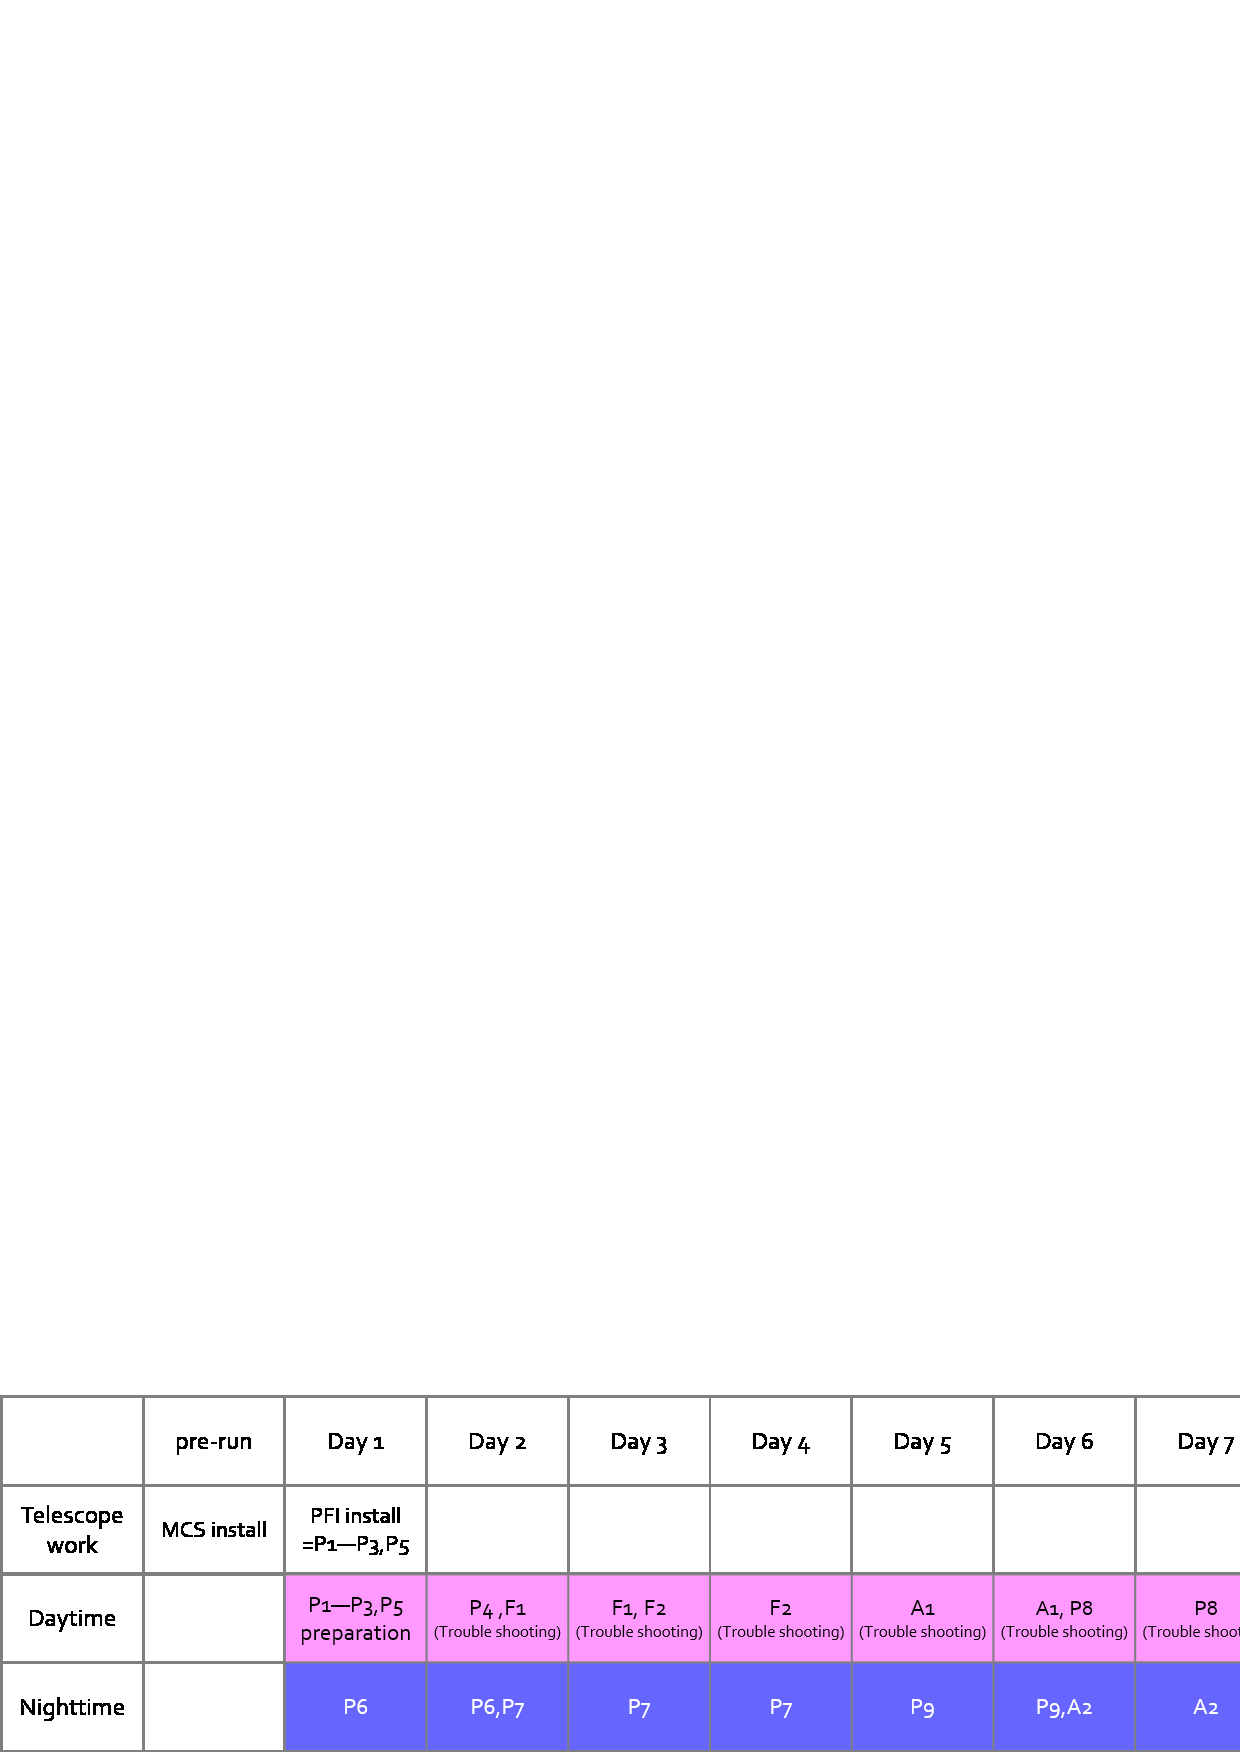
\includegraphics[width=108mm]{timetable_run2.pdf}
	\end{center}
	\vspace*{-5mm}
	\caption{Time table of Run 2.}
	\label{fig:run2}
\end{minipage}
\end{tabular}
\end{center}
\end{figure}

%---------------------------------------------------
% Run 3
%---------------------------------------------------
\begin{figure}[!ht]
\begin{center}
\begin{tabular}{c}
\begin{minipage}{0.95\hsize}
\paragraph{Run 3 : 10 days  (Figure \ref{fig:run3})}
During the telescope down-time for Mitsubish's test using PFS, we will use the nights to test Cobra using MCS. 
	\begin{itemize}
	\item 1 day (daytime) for P-1 -- P-3,  and F-1:
	(1) check PFI/POpt2 standing by,
	(2) install POpt2 to the prime focus,
	(3) check PFI functions, and
	(4) connect Cable B to PFI and SpS (SM1)
	\item 0.5 day (nighttime) for P-4 :
	(1) verify  MCS performance at zenith
	\item $\sim 5$ days (nighttime) for A-1 :
	(1) calibration of Cobras (all)
	\item $\sim 2$ days (1.0-day nighttime) for A-2 : 
	(1) PSF measurement through the entire system (SM1)	
	\item 1 day (nighttime) for P-4 and P-5 (after telescope can be moved):
	(1) measure x/y offset of PFI rotation center on MCS, and
	(2) verify  MCS performance at different elevation angle
	\end{itemize}
We also plan to take arc and flat images.
\end{minipage} \\
\begin{minipage}{0.8\hsize}
	\begin{center}
	\vspace*{5mm}
	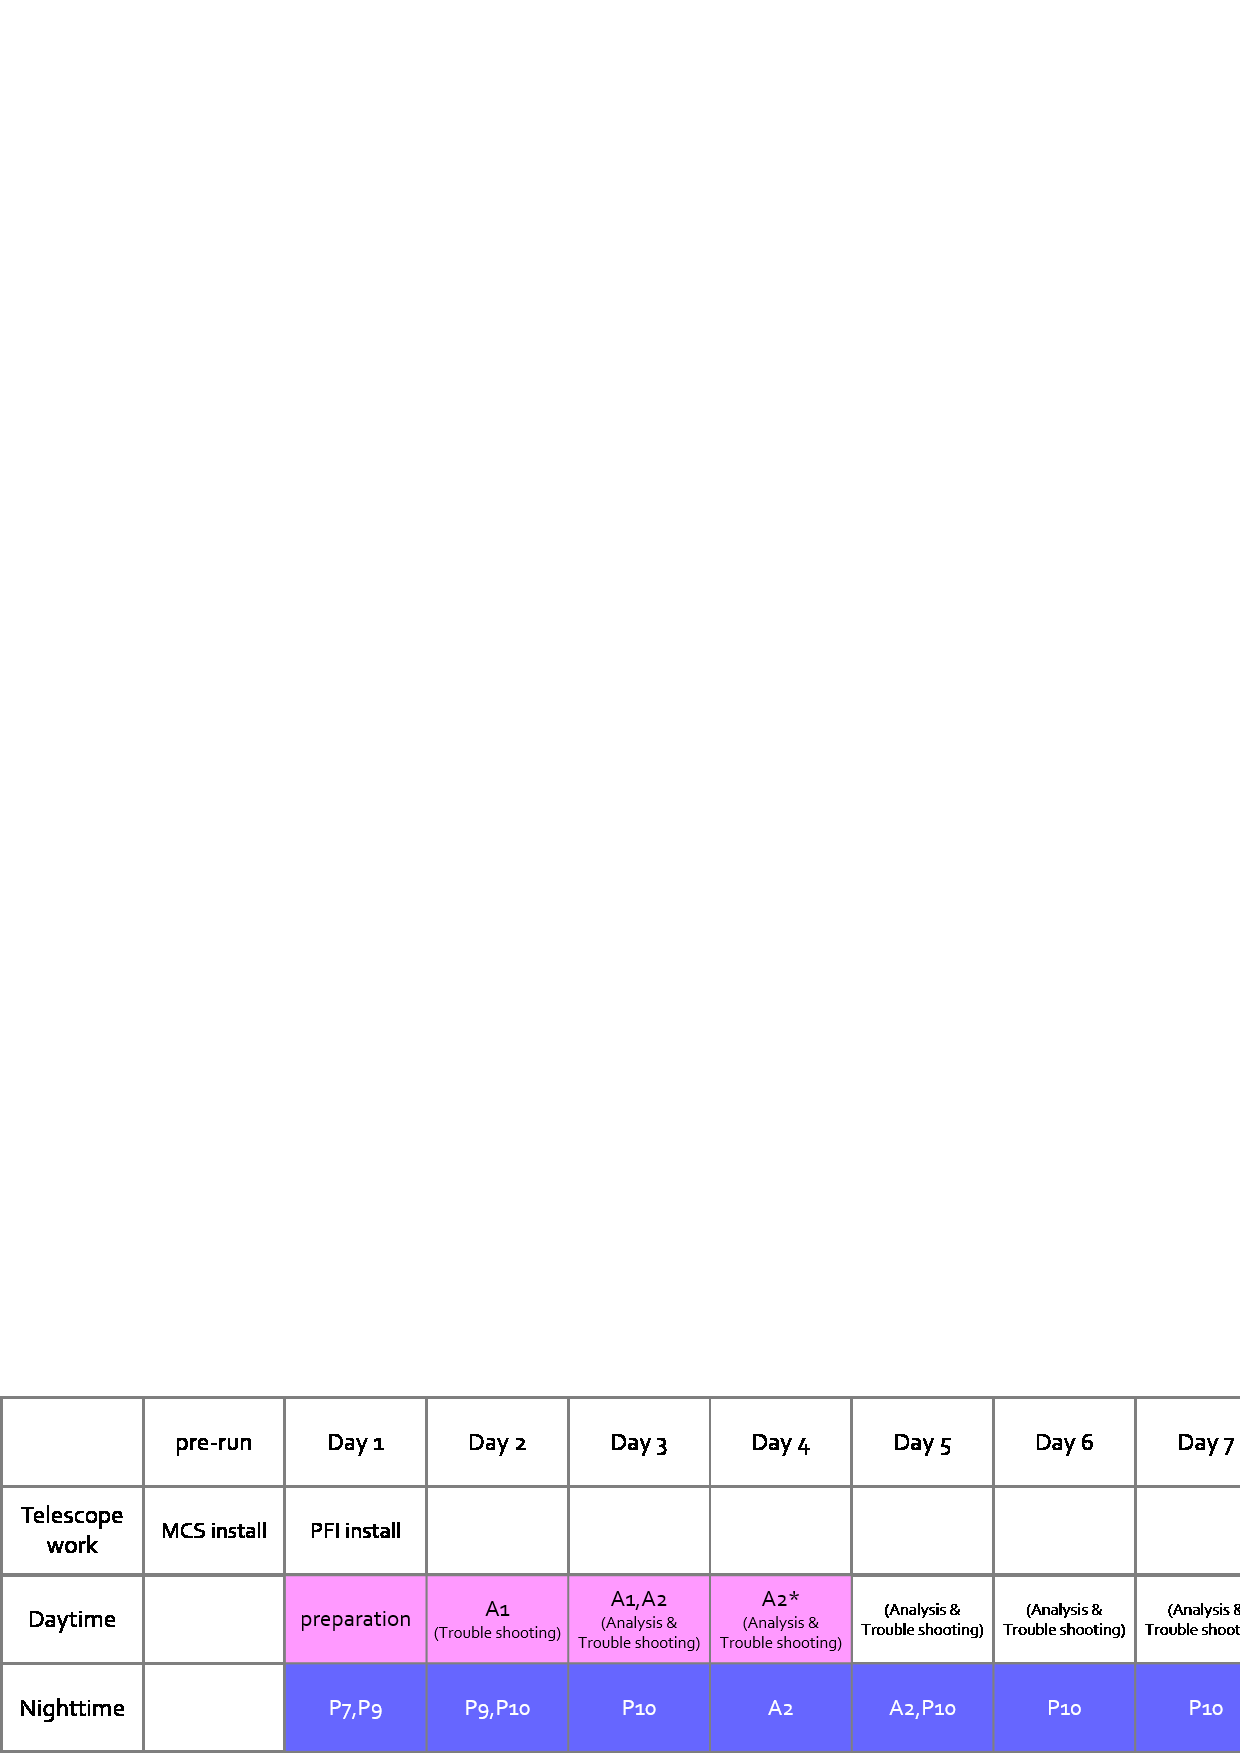
\includegraphics[width=120mm]{timetable_run3.pdf}
	\end{center}
	\vspace*{-5mm}
	\caption{Time table of Run 3.}
	\label{fig:run3}
\end{minipage}
\end{tabular}
\end{center}
\end{figure}


%---------------------------------------------------
% Run 4
%---------------------------------------------------
\begin{figure}[!ht]
\begin{center}
\begin{tabular}{c}
\begin{minipage}{0.95\hsize}
\paragraph{Run 4 : 7 days  (Figure \ref{fig:run4})}
	\begin{itemize}
	\item 1.2 $+$ 1.5 days (nighttime) for P-6 :
	(1) verification of A\&G camera functions (1.5 days is done with Mitsubishi)
	\item 1.0 days (nighttime) for P-7 :
	(1) correct WFC shift/tilt with respect to the primary mirror
	\item 1.5 days (daytime) for P-8 :  
	(1) confirm fixed fiducial fiber positions on F3C (refine the PFI-MCS relation)
	\item 1,5 days (nighttime) for P-9 :
	(1) Telescope Pointing Analysis (w/ith Mitsubishi)
%	\item 0.7 day (daytime) for F-1 : 
%	(1) connect Cable B to PFI and SpS (SM1/2/3)
	\item 0.5 days (daytime and/or nighttime) for A-1 : 
	(1) Test fiber allocation
	\item 1.0 days (1.0-day nighttime) for A-2 : 
	(1) PSF measurement through the entire system (SM1,2,3)	
\end{itemize}
The run 4 has 3-night work by/with Mitsubishi for test of software of the telescope control.
Note that we assume that we can coordinate with Mitsubishi to proceed some test items in parallel.
Note also that some test items such as AG functionality test and TPA will be done with Mitsubishi. 
The below is test items when we apply the engineering time in the S21B semester:
\begin{verbatim}
[a] POpt2 alignment, measure InR center using AG camera. [1 night]
[b] AG camera test and characterization [1.2 nights]
    - AG camera centroiding test (0.3 nights)
    - AG camera Orientation and pixel scale measurement (0.3 night)
    - Check focus position of AG focal plane and focusing test (0.4 night)
    - Field acquisition (0.2 night)
[c] Mitsubishi's test for AG [1.5 nights]
[d] Mitsubishi's test for PA [1.5 nights]
[e] Fiber allocation test [0.5 nights]
[f] PSF characterization for development of data reduction pipeline [1 night]
    - Sky spectra acquisition at different El and InR (0.5 nights x 2 sets). 
        (2 sets of images are needed to study time dependency)

    Note: In addition to night-time observation, the following tests need to be 
          done at the daytime. 
    - Measurement of PFI rotation center on MCS and check the repeatability 
      of installation. (0.1 day)
    - Check and refine the fixed fiducial fibers position on focal plane. (1 day)
    - Study effect of the Cobra position on PSF (0.5 day x 4 sets) 
\end{verbatim}
\end{minipage} \\
\begin{minipage}{0.8\hsize}
	\begin{center}
	\vspace*{5mm}
	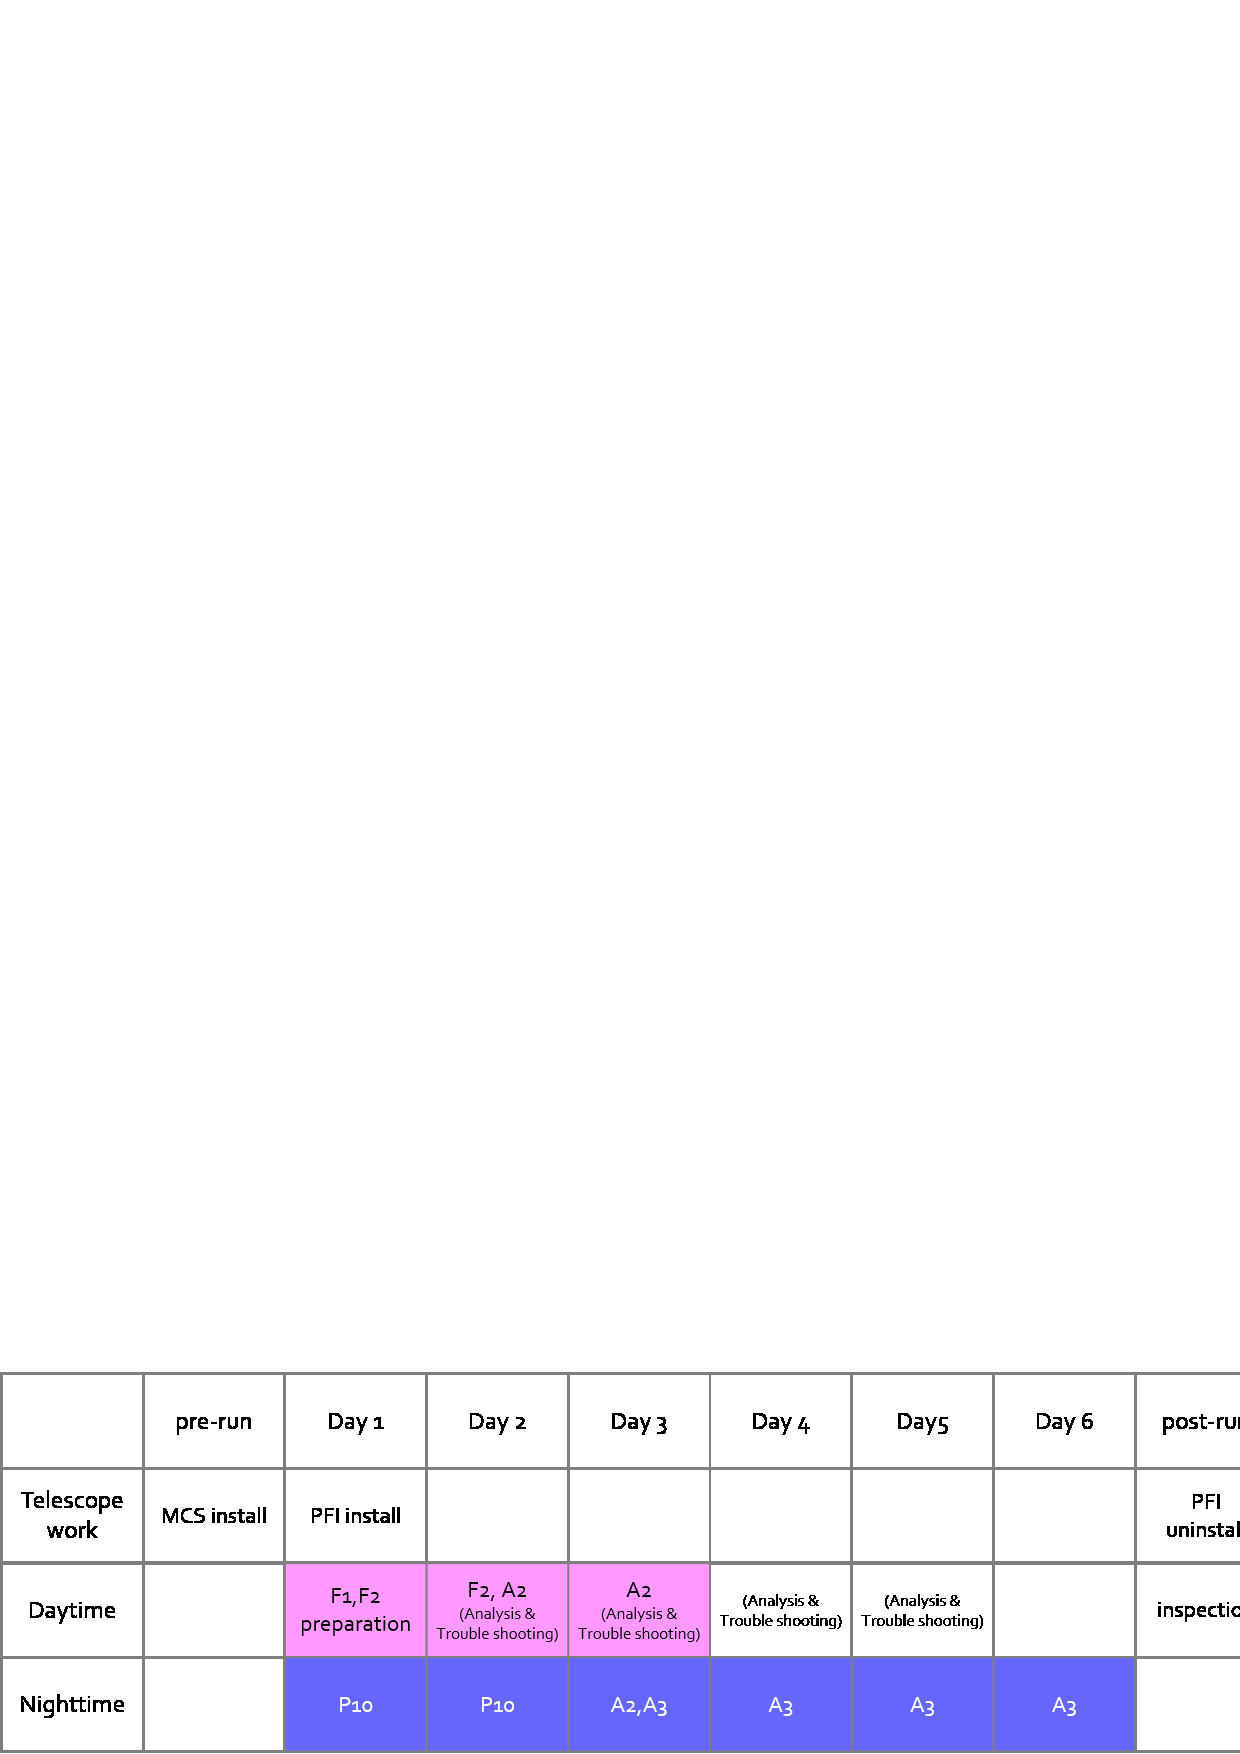
\includegraphics[width=120mm]{timetable_run4.pdf}
	\end{center}
	\vspace*{-5mm}
	\caption{Time table of Run 4.}
	\label{fig:run4}
\end{minipage}
\end{tabular}
\end{center}
\end{figure}

%---------------------------------------------------
% Run 5
%---------------------------------------------------
\begin{figure}[!ht]
\begin{center}
\begin{tabular}{c}
\begin{minipage}{0.95\hsize}
\paragraph{Run 5 : 5 days  (Figure \ref{fig:run5})}
	\begin{itemize}
	\item 0.2 days (nighttime) for P-6 :
	(1) check AG focus comparing with the focus of the science fibers.
	\item 0.3 days (nighttime) for P-7 :
	(1) correct WFC shift/tilt with respect to the primary mirror (confirmation)
	\item 0.1 days (nighttime) for P-9 :
	(1) Telescope Pointing Analysis (confirmation)
	\item 2 days (nighttime) for P-10 : 
	(1) 1st-pass distortion map
	\item 2.5 days (1.0-day daytime and 1-day nighttime) for A-2 : 
	(1) PSF measurement through the entire system (SM1)
	\item 1 day (nighttime) for A-3 : 
	(1)2nd-pass distortion map
	\end{itemize}
%If needed, we will connect SM1 to the Cable B for other Spectrograph Modules to see spatial variation for test \ref{secflow:PSFchar}
The below is test items when we apply the engineering time in the S21B semester.
Since 5 nights are allocated whereas 7 nights were applied, 1 nights are reduced for A-10 and A-3, respectively:
\begin{verbatim}
[a] POpt2 alignment and InR center confirmation (repeatability) [0.3 nights]
[b] Confirm telescope pointing [0.1 nights]
[c] Determine the AG camera coordinate system w.r.t. the fiducial fibers [1.5 nights] 
    - dithering around the AG fiducial fibers (2 fibers for each camera). 
    - El dependency confirmation
[d] Distortion study using astrometry data on AG camera [3 nights]
    - Study dependency of the instrument rotator
    - Study dependency on elevation
    - Study dependency on ADC position
      In total, ~50  set of data (1 set ~0.05 nights)
[e] Distortion study by taking star spectra (dithering around the allocated 
    position) [2 nights]
    - Do dithering (raster-scan) for ~20 fields at different El, N/S and InR and 
      refine fiber allocation. (0.1 nights per field)
[f] AG focus position measurement to compare with the science fibers focal plane 
    [0.2 nights]
[g] Take reference star spectra (radial velocity standard, telluric, abundance) for 
    data reduction pipeline [0.5 night]
[h] PSF characterization for development of data reduction pipeline [1 night]
    - Sky spectra acquisition at different El and InR  (0.5 nights x 2 sets)

    Note: In addition to night-time observation, the following tests need to be 
          done at the daytime. 
   - Study effect of the Cobra position on PSF (repeatability) (0.25 day x 4 sets) 
\end{verbatim}
\end{minipage} \\
\begin{minipage}{0.8\hsize}
	\begin{center}
	\vspace*{5mm}
	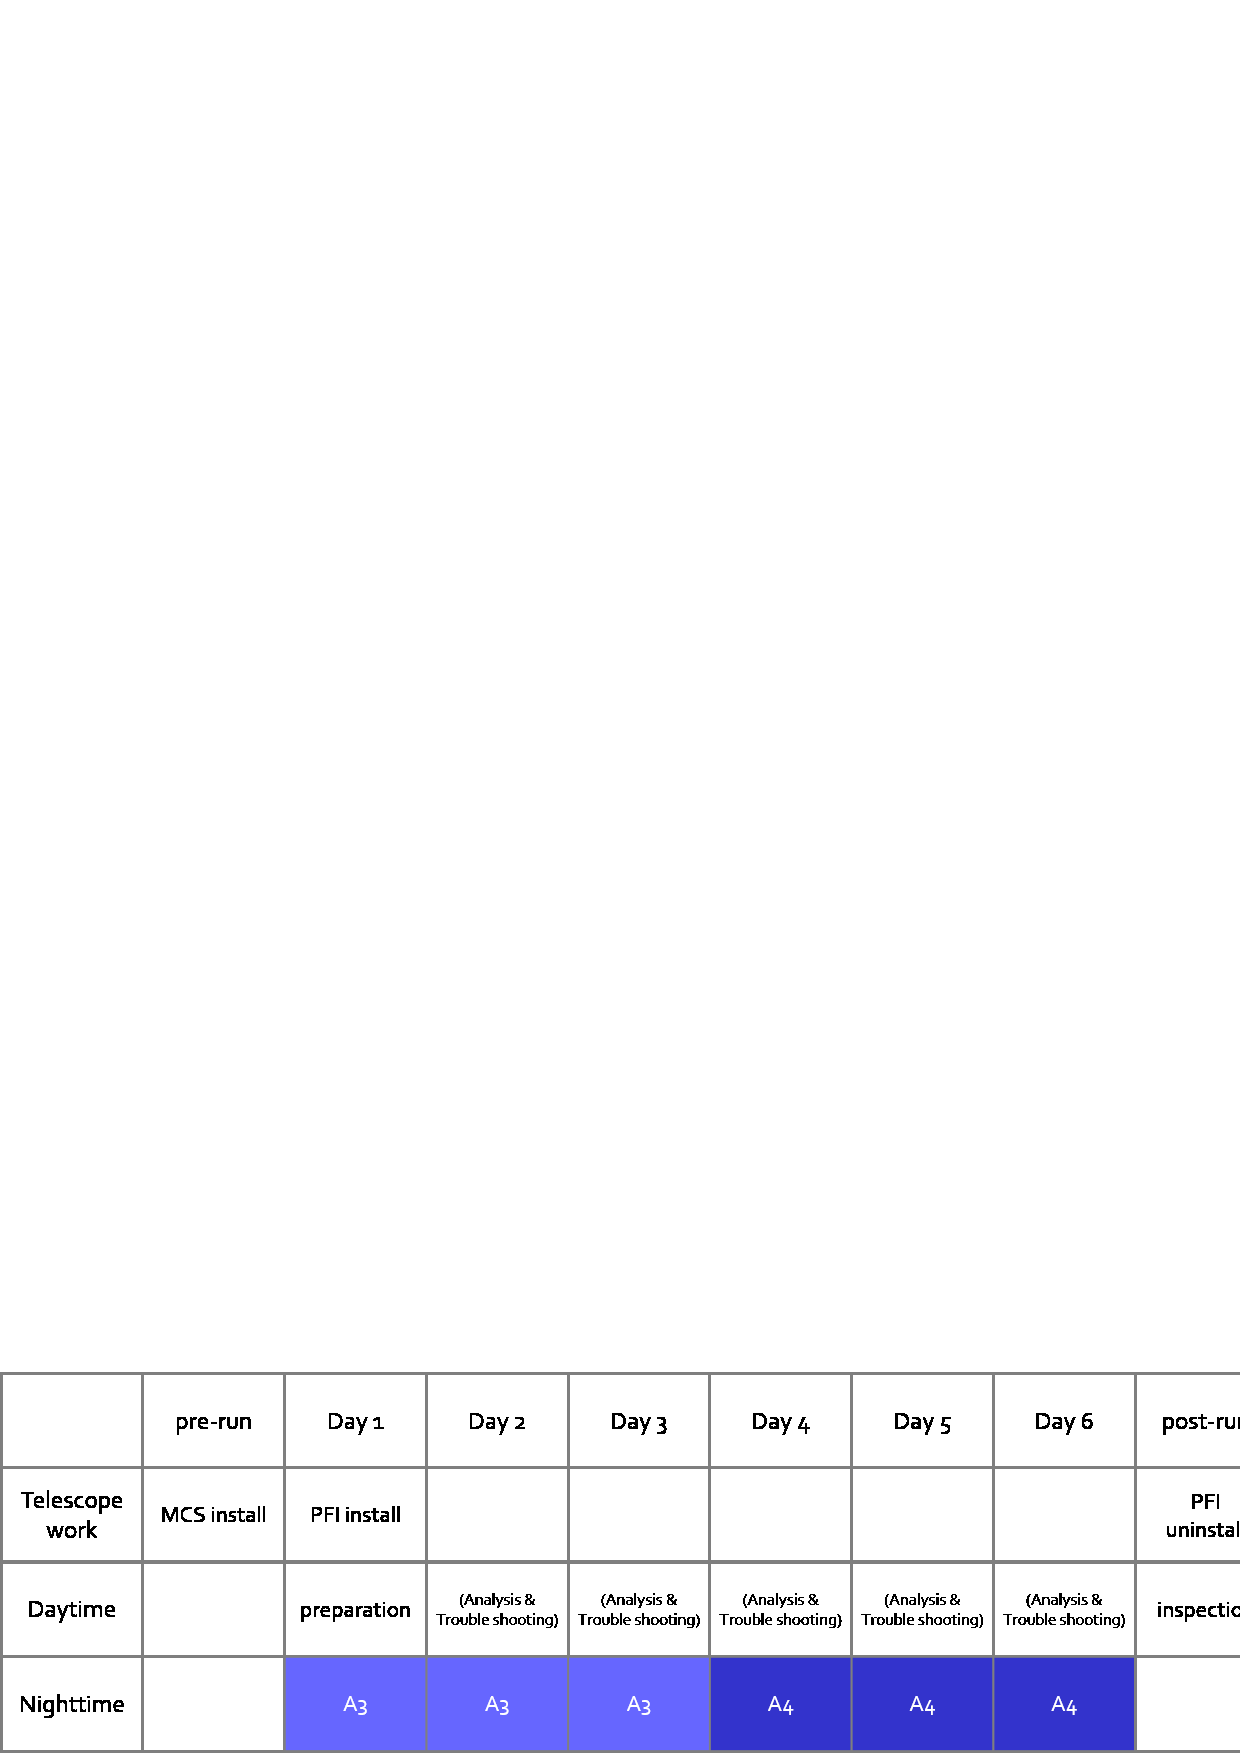
\includegraphics[width=98mm]{timetable_run5.pdf}
	\end{center}
	\vspace*{-5mm}
	\caption{Time table of Run 5.}
	\label{fig:run5}
\end{minipage}
\end{tabular}
\end{center}
\end{figure}

%---------------------------------------------------
% Run 6
%---------------------------------------------------
\begin{figure}[!ht]
\begin{center}
\begin{tabular}{c}
\begin{minipage}{0.95\hsize}
\paragraph{Run 6 : 6 days  (Figure \ref{fig:run6})}
	\begin{itemize}
	\item 2 days (nighttime) for P-10 : 
	(1) 1st-pass distortion map
	\item 0.5 day (daytime) for F-1 :  
	(1) connecting Cable B to PFI and SpS (SM2,3,4)
	\item 1.0 day (daytime) for F-2 :  
	(1) confirmation of  the fiber identifications (SM2,3,4)
	\item 1.5 days (1.0-day daytime and 0.5-day nighttime) for A-2: 
	(1) PSF measurement through the entire system (all but SM4-NIR)
	\item 3.5 days (nighttime) for A-3: 
	(1) 2nd-pass distortion map
	\end{itemize}
% If needed, we will connect SM1 to the Cable B for other Spectrograph Modules to see spatial variation for test \ref{secflow:raster}
\end{minipage} \\
\begin{minipage}{0.8\hsize}
	\begin{center}
	\vspace*{5mm}
	\includegraphics[width=108mm]{timetable_run6.pdf}
	\end{center}
	\vspace*{-5mm}
	\caption{Time table of Run 6.}
	\label{fig:run6}
\end{minipage}
\end{tabular}
\end{center}
\end{figure}


%---------------------------------------------------
% Run 7
%---------------------------------------------------
\begin{figure}[!ht]
\begin{center}
\begin{tabular}{c}
\begin{minipage}{0.95\hsize}
\paragraph{Run 7 : 6 days  (Figure \ref{fig:run7})}
	\begin{itemize}
	\item 4 days (nighttime) for A-3: 
	(1) 2nd-pass distortion map
	\item 2 days (dark-night) for A-4 :
	(1) performance verification I (all but SM4-NIR)
	\end{itemize}
\end{minipage} \\
\begin{minipage}{0.8\hsize}
	\begin{center}
	\vspace*{5mm}
	\includegraphics[width=108mm]{timetable_run7.pdf}
	\end{center}
	\vspace*{-5mm}
	\caption{Time table of Run 7.}
	\label{fig:run7}
\end{minipage}
\end{tabular}
\end{center}
\end{figure}

%---------------------------------------------------
% Run 8
%---------------------------------------------------
\begin{figure}[!ht]
\begin{center}
\begin{tabular}{c}
\begin{minipage}{0.95\hsize}
\paragraph{Run 8 : 5 days  (Figure \ref{fig:run8})}
	\begin{itemize}
	\item 2.0 days (1.0-day daytime and 1.0-day nighttime) for A-2: 
	(1) PSF measurement through the entire system (all SMs)
	\item 4 days (dark-night) for A-4 and A-5 : 
	(1) performance verification I (SM1/2/3),  and
	(2) performance verification II (stabilization, using SM1/2/3)
	\end{itemize}
\end{minipage} \\
\begin{minipage}{0.8\hsize}
	\begin{center}
	\vspace*{5mm}
	\includegraphics[width=98mm]{timetable_run8.pdf}
	\end{center}
	\vspace*{-5mm}
	\caption{Time table of Run 8.}
	\label{fig:run8}
\end{minipage}
\end{tabular}
\end{center}
\end{figure}

%---------------------------------------------------
% Run 9 and 10
%---------------------------------------------------
\begin{figure}[!ht]
\begin{center}
\begin{tabular}{c}
\begin{minipage}{0.95\hsize}
\paragraph{Runs 9 and 10 : 4 days  (Figure \ref{fig:run9})}
	\begin{itemize}
	\item 4 days (dark-night) for A-5 :
	(1) performance verification II (stabilization)
	\end{itemize}
\end{minipage} \\
\begin{minipage}{0.8\hsize}
	\begin{center}
	\vspace*{5mm}
	\includegraphics[width=84mm]{timetable_run9.pdf}
	\end{center}
	\vspace*{-5mm}
	\caption{Time table of Runs 9 and 10.}
	\label{fig:run9}
\end{minipage}
\end{tabular}
\end{center}
\end{figure}


%--------------------------------------------------------------
%  Table: expected runs and nights
%--------------------------------------------------------------
\setlength{\tabcolsep}{1mm}{
\begin{table}[!ht]
\begin{center}
\caption{
Expected number of working days for commissioning (as of June 2021).
Column 1 lists the run number.
Year/Month in column 2 are just roughly set  for the Run 6 and later assuming the latest schedule of each subsystems and that scientific operation will start in the S23B  semester.
The required days for each run are listed in column 3.
Required days for individual  processes at each run are listed in column 5 (daytime) or 6 (night-time).
The numbers in parentheses in column 6 is required dark nights.  
}
%\scriptsize
\footnotesize
\begin{tabular}{*{3}{c}|*{3}{c}}\label{tbl:CountDates} \\ \hline
Run	 & Year/Month  &\#days & process	& daytime & night (dark) \\ \hline \hline
0	& S17B--S21A			& 4.5***	& P7(*) etc.	& 0		& 7.0 (2.5)	\\ \hline
--	& 2018/06			& --		& M1		& --		& --	\\ \hline
1	& 2018/10			& 3		& M1--3		& (1**)	& 0	(0)	\\
	& 	& 				& M4, ASIAA	& 0		& 3	(0)	\\ \hline
2	& 2019/08	& 5				& M4, M3, ASIAA	& 0		& 5	(0)	\\ \hline
--	& 2019/12--2020/01			& --		& S1,S2 (SM1:B+R)		& --		& --	\\ \hline
3	& 2021/09	& 10****			& P1--P3,F1 (SM1)	& 	& 0.5 (0)	\\
	&	&					& P4,P5			& 0 	& 1.5 (0)	\\
	&	&					& A1	& 0 	& 5.0 (0)	\\
	&	&					& A2 (SM1B+R)	& 0 	& 2.0 (0)	\\ \hline
4	& 2021/10	& 7***			& P6  			& 0 	& 2.7*** (0)	\\
	&	&					& P7  			& 0 	& 1.0 (0)	\\
	&	&					& P8  			& 1.5 	& 0 (0)	\\
	&	&					& P9  			& 0 	& 1.5*** (0)	\\
	&	&					& A1	& 0.5 	& 0 (0)	\\
	&	&					& A2 (SM1,2,3)	& 0 	& 1.0 (0)	\\ \hline
5	& 2021/11	& 5 		& P6 			& 0 	& 0.2 (0)	\\
	&	&					& P7 			& 0 	& 0.3 (0)	\\
	&	&					& P9  			& 0 	& 0.1 (0)	\\
	&	&					& P10  			& 0 	& 2 (0)	\\
	&	&					& A2 (SM1)	& 1 	& 1 (0)	\\ 
	&	&					& A3 			& 0 	& 1 (0)	\\ \hline
--	& 2022/early			& --		& S1,S2 (SM2:B+R)		& --		& --	\\ 
--	& 2022/early			& --		& S1,S2 (SM3)		& --		& --	\\ 
--	& 2022/early			& --		& S1,S2 (SM4:B+R)		& --		& --	\\
--	& 2022/middle			& --		& S1,S2 (SM1:N)		& --		& --	\\ \hline
6	& 2022/05	& 6 		& P10 			& 0 	& 2 (0)	\\
	&	&					& A2 (SM1,2,3)	& 1 	& 0.5 (0)	\\
	&	&					& A3 			& 0 	& 3.5 (0)	\\ \hline
--	& 2022/middle			& --		& S1,S2 (SM2:N)		& --		& --	\\ \hline
7	& 2022/07	& 6					& A3			& 0		& 4 (0)	\\
	&	&					& A4			& 0		& 0 (2)	\\ \hline
--	& 2022/07			& --		& S1,S2 (SM4:N)		& --		& --	\\ \hline
--	& 2022/middle			& --		& S1,S2 (SM4:N)		& --		& --	\\ \hline
8	& 2022/10	& 5			& A2 (all SMs)	& 1 	& 1 (0)	\\
	&	&					& A4			& 0		& 0	(2)	\\
	&	&					& A5			& 0		& 0 (2)	\\ \hline
9	& 2022/12	& 4			& A5			& 0		& 0 (4)	\\ \hline
19	& 2023/02	& 4			& A5			& 0		& 0 (4)	\\ \hline \hline
\multicolumn{2}{r}{in total}& 45 (52***) \\ \hline
\end{tabular}
\\
* Check algorithm at HSC engineering run. \\
** Telescope can be used for other instruments \\
*** The number combined with run 0 and Mitsubishi's work \\
**** During telescope downtime for Mitsubishi's test (the number of used night is not counted)
\end{center}
\end{table}

\clearpage

\subsection{Relationship among Individual Sequence}
Some processes can be carried out in parallel, but some should in series.
Table \ref{tbl:Rel_Seq} shows the relationship among the individual sequences.
Each row displays commissioning processes related to each process in the columns.
``X" means required process.
For example, prior to the process M--3, M--2 (and hence M--1) should be succeeded.

%--------------------------------------------------------------
%  Table: the relation ship of commissioning sequence 
%  A sequence (top) marked with X is need prior to other sequence (row)
%--------------------------------------------------------------
\begin{table}[!ht]
\caption{
The relation of commissioning processes.}
\label{tbl:Rel_Seq}
\begin{center}
\includegraphics[width=170mm]{relationship_sequences.eps}
\end{center}
\end{table}




% Section: Details of Procedure
\section{Details of Work Flow}

% MCS part
\renewcommand{\thesubsubsection}{M-\;\arabic{subsubsection}}
\subsection{Validation of MCS}\label{sec:MCS}
%%%%%%%%%%%%%%%%%%%%%%%%%%%%%%%%%%%%%%%%%%%%
\subsubsection{Off-Telescope (stand-by) characterization of MCS [Daytime]}\label{secflow:MCSoff}
In this step, the basic functions of MCS are checked before installation to the telescope.

Firstly, we turn on the power of MCS computer and electronic chassis.
Then we check the following functions:

\begin{itemize}
\item MCS can read CMOS sensor with expected performance.
	\begin{itemize}
	\item dark level: No detectable dark current at 20--25 [decC] with 1.1 sec. exposure time
	\item noise level: $6.4 e^-$
	\item background level: \redtext{how much??}
	\item shutter: We take several images changing the exposure time to confirm the mechanical shutter works properly.
	\end{itemize}
These values are cited from the CDR slides ({\tt MCS camera system.pdf}).
\item MCS can read environmental and mechanical (?) sensors.
	\begin{itemize}
	\item 7 temperature sensors \redtext{(where)?}
	\item \redtext{flow meter?}
	\end{itemize}
\end{itemize}

In addition, we will send command on Subaru side (Gen2), so that we can validate ICS performance as follows:
\begin{itemize}
\item MHS communicates with between Gen2
\item IIC interprets Gen2 commands and send MCS proper commands through MHS
\item Subaru (STS and Gen2) refers MCS status 
\item Subaru (Gen2) receives MCS image
\end{itemize}
%Because every command is sent vis MHS, we can confirm communication via MHS in this sequence. 
%That is we also validate that MHS can send commands to read CMOS sensors and environmental sensors, and then receive proper results and status.

%Besides, MCS should be characterized in off-telescope condition, such as temperature, noise-level and so on.

Note that once MCS is powered on, it will be connected to the power supply and Subaru network.
The telemetry is monitored during stand-by.
Considering this fact, we can skip this step from the second and more times for commissioning run.

After validating the above performance, we will take calibration data (bias, dark, and flat) of CMOS sensor.
Note that this process will be skipped in this step, and be carried out in the step \ref{secflow:MCSon} instead.

\paragraph{Designated Tool for this step}
We will prepare commands to check MCS functions.
This will be used as health check of the subsystem.

\begin{itembox}[l]{\suctitle{Success Criteria}}
All MCS basic functions are verified --- power, CMOS sensor, telemetry. \\
ICS can control the instrument communicating with Gen2.

\bluetext{Required long time to analyze the data?: No. \\
---We can check the functions in real time.}
\end{itembox}
%%%%%%%%%%%%%%%%%%%%%%%%%%%%%%%%%%%%%%%%%%%%
\subsubsection{MCS installation to the Telescope [Daytime]}\label{secflow:MCSinstall}

In this process, MCS is installed to the Cassegrain (Cs) Focus of the Subaru telescope.
MCS is attached to MCBox, which is installed to the flange of the Cs focus. 
This means that the MCS position is determined by how accurate MCBox is attached to the Cs focus.
The requirement {\tt REQ-MET-9} demands the accuracy of the MCS position with respect to the optical axis; decenter within 45mm (x/y each), and tilt within 0.14 degree.
Subaru demonstrated the repeatability of mounting MCBox in 2015 (report by Y. Minowa: {\tt NDTN-20150714}\footnote{MCBox\_repeatability\_report.pdf}), resulting in the following performance:
\begin{itemize}
\item Tilt: $<$ 10 arcsec
\item Shift(X,Y): $<$ 50um
\item Shift(Z): $<$ 0.5mm
\item Rot. : 0.0015 degree (shift by 0.24 um at the edge of MCS FoV)
\end{itemize}
This result implies the MCS will be installed well within the required accuracy, if it is installed in the normal way.
Note that we don't measure the repeatability indeed in the commissioning processes.
We will, however, have to check this process later, when a problem will happen; e.g. the center of PFI on MCS are quite different in individual runs.

%\bluetext{
%In this step, it should be also confirmed that flange, I/F of MCBox and M1, and CMOS sensor is parallel (Fig. \ref{fig:MCSinst}).
%This is needed to measure PFI z offset/tilt (see section \ref{secflow:P05})
%}

%In the different run, the repeatability of mounting MCBox can be measured mechanically (is it needed again?).

%\begin{figure}[!ht]
%\begin{center}
%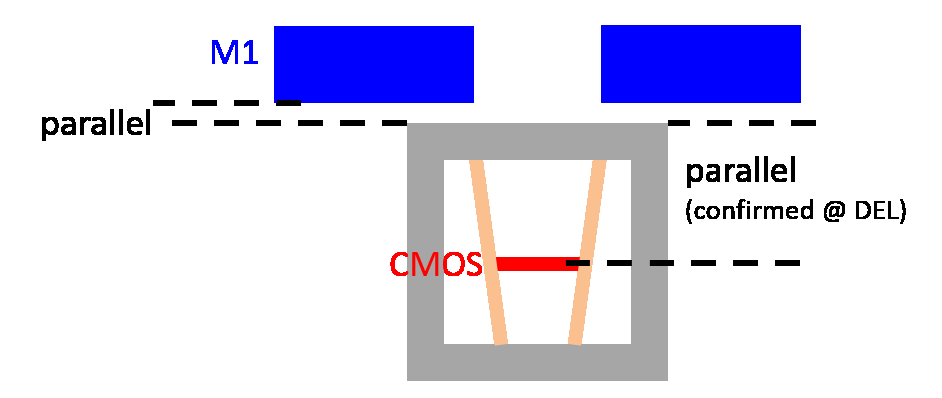
\includegraphics[width=100mm]{MCSinstall.eps}
%\end{center}
%\caption{Sketch of MCS installation}
%\label{fig:MCSinst}
%\end{figure}

% This requirement is not needed any more, because z offset of PFI cannot be measured using MCS image
%\bluetext{
%Additional requirement before shipment:
%The top part of MCS arm and CMOS sensor should be parallel (or angle should be measured).
%}

\begin{itembox}[l]{\suctitle{Success Criteria}}
MCS is mounted to Cassegrain focus with the required accuracy ($\leq$ 45mm offset in x/y direction, and $\leq$ 0.14 degree tilt). 

\bluetext{Required long time to analyze the data?: No.}
\end{itembox}
%%%%%%%%%%%%%%%%%%%%%%%%%%%%%%%%%%%%%%%%%%%%
\subsubsection{Check of Basic Functions of MCS on the Telescope [Daytime]}\label{secflow:MCSon}

\milestone{MCS is operated on the telescope for the first time.}

After installation to the telescope, basic functions of MCS are checked again, but on-telescope condition in this process.
During installing operation, the power of MCS will be kept on (TBC\footnote{Having UPS, MCS computer can be kept on. Still, the network will be disconnected}), so we should turn on the MCS electric devices (or reconnect to the network) again.

Then we check the following functions (the same as \ref{secflow:MCSoff}):

\begin{itemize}
\item MCS can read CMOS sensor with expected performance.
	\begin{itemize}
	\item dark level: No detectable dark current at 20--25 [decC] in one 0.8s frame
	\item noise level: $6.4 e^-$
	\item background level: \redtext{how much??}
	\item shutter: We take several images opening and closing the mechanical shutter to confirm it works properly.
	\end{itemize}
These values are cited from the CDR slides ({\tt MCS camera system.pdf}).
\item MCS can read environmental sensors.
	\begin{itemize}
	\item 7 temperature sensors on optics, mechanical structure, coolant lines, MCBox and electrical rack \redtext{(where exactly?)}
	\item flow meter
	\item microphone
	\end{itemize}
\end{itemize}

After the basic functions are confirmed to work, the calibration data (flat, bias and, dark?:TBC) of CMOS sensor shall be obtained, if they are not taken in the step of \ref{secflow:MCSoff}.
The stability of calibration data can be examined using the data in multiple runs.

\paragraph{Designated Tool for This Process}
We will prepare commands to check MCS functions, the same as \ref{secflow:MCSoff}.

%By sending command from gen2, we will also confirm communication between MCS and Gen2.

%\redtext{
%According to the MCS delta-CDR, the flat screen is attached MCS flange for obtaining flat-fielding, and 3--4 LEDs are attached near MCS-M1 module.
%On the other hand, because the Cassegrain stand-by flange has a space for light source on the top, the calibration data can be obtained during stand-by (TBD).
%}

\begin{itembox}[l]{\suctitle{Success Criteria}}
All MCS basic functions are verified --- power, CMOS sensor, telemetry.  \\
The calibration data (bias, flat, and dark?) of CMOS are acquired.

\bluetext{Required long time to analyze the data?: No. \\
--- We can check the functions in real-time}
\end{itembox}


%%%%%%%%%%%%%%%%%%%%%%%%%%%%%%%%%%%%%%%%%%%%
\subsubsection{Verify MCS performance [Daytime]}\label{secflow:prestudy}
In this sequence, we verify MCS performance to measure the fiber positions on focal plane.
We also check validity the PFS coordinate-transfer system.
Here, because MCS will arrive prior to PFI arrival\footnote{ASIAA also propose that MCS be aligned with the prime focus using pinhole array on POpt2 or FMOS/PIR, which is required after PFI arrival.}, there are two options for this test.
One is FMOS/PIR instead of fiber positioner system, and the other is pinhole array equipped to POpt2.

\paragraph{In the case of FMOS/PIR}
The field of view of FMOS ($\sim 30$ arcmin in diameter) is much smaller than that of PFS.
Besides, only 32 fibers can be back-illuminated simultaneously.
Nonetheless, the procedure of coordinate transformation shall be studied well.

MCS measures fiber positions somewhat converted to MCS frame, and then positions are transferred to them on focal plane.
On the other hand, FMOS fiber positioner (Echidna) measures fiber positions on the focal plane.
By comparing measured fiber positions by MCS and the coordinate transformation system, with those by Echidna, MCS function of measuring the fiber positions is verified.
%The error in measurement contributed by dome seeing temperature, or telescope elevation will be also estimated by measuring position several elevation and temperatures.
%% estimation of error is needed for PFI-MCS relation? maybe not. but error estimation is needed for measurement on MCS?
%% Echidna: 20 fibers are illuminated at a time
At present, Echidana can position fibers with the accuracy of $\sim 35$ um\footnote{Originally the fiber allocation was achieved with the accuracy of $\sim 10$um. Recently the encoder of X position of sky camera was broken, which have added $\sim 25$ um for fiber positions.}.
We set the goal in accuracy of fiber positioning 50 um for pre-study, the same as 1-st pass distortion map (\ref{secflow:1stDM}).

The procedure of the measurement is as follows:
\begin{enumerate}
\item Decide which fibers to move and which fibers not to move (like fixed fiducial fibers).
Figure \ref{fig:fibEchidna} shows an example.
%One way is to define  nine fixed fibers arranging 3 $\times$ 3 grid. 
\item Built distortion map of PIR from the MCS viewpoint (the form of $D_2$ for FMOS/PIR).
With all fibers back-illuminated, we take the fiber image at home position by MCS.
We also have the physical positions of FMOS fibers.
Using these positions, we will determine the form of the distortion map.
\item Define F3C for FMOS. 
In order to distinguish with F3C for PFS, we name the defined coordinate ``F3C(PIR)". 
``F3C(PIR)" is practically the same as the positions measured with the spine camera of Echidna.
With fixed fibers back-illuminated, we take fibers image by both MCS and Echidna, and then the positions of fixed fiducial fibers on F3C are measured.
\item Take all fibers image by MCS and calculate their position
\begin{enumerate}
\item Using image of fixed fibers, determine the transformation from MCS coordinate to F3C(PIR) coordinates, that is, the parameters of $D_2$ for FMOS/PIR). 
\item Using images of the rest fibers, calculate the positions on above coordinate frame.
\end{enumerate}
\item Measure fiber positions of FMOS/PIR, and compare with those derived on F3C(PIR)
\item Executing the above procedures for several fiber configurations at a various Elevation (EL) and Rotator angle (ROA), study the stability of the measurements.
\redtext{We may be able to study the effect of local surface error of corrector lens for coordinate transform by changing fiber configurations.} 
Here the error due to temperature and dome seeing is included.
We also examine these effect.
\end{enumerate}

%--------------------------------------------------------------
%  Figure: An example of fiber arrangement 
%--------------------------------------------------------------
\begin{figure}[!ht]
\begin{center}
\includegraphics[width=100mm]{fiber_echidna.eps}
\end{center}
\caption{
Example of the arrangement of FMOS/Echidna back-lit fibers.
32 fibers can be back-illuminated at a time. }
\label{fig:fibEchidna}
\end{figure}

\paragraph{In the case of pinhole array on POpt2}
If pinhole array can be attached on the POpt2, we can study transfer coordinate system in the similar procedure above.
WFC has a ring-patterned local surface error with a pitch of 6mm, pinholes with the smaller pitch enable us to study the effect of the local surface error.
Using pinholes are arranged at fiducial fiber position and hexagonal position of 4 mm (half size of that of cobras), we will study the the coordinate transform in the following procedure.
\begin{enumerate}
\item Distortion map is determined with WFC as-built model.
\item \label{item:M4pin2} Take pin holes array images by MCS.
Choose one of the holes in the patrol areas and calculate their position on F3C.
\item Compare the calculated positions with the design.
\item Choosing the another holes, repeat \ref{item:M4pin2}.
\item Executing the above procedures at a various Elevation (EL) and Rotator angle (ROA), study the stability of the measurements.
\end{enumerate}

Because the corrector lens are different between PIR and WFC, we cannot study a effect of WFC itself if we use FMOS.
However, similar study will be performed by changing the fiber configurations (TBC).


\paragraph{Back-up plan}
If MCS would deliver at Subaru just before the arrival of PFI, we will not have enough time to practice the procedure of the coordinate transformation.
As back-up plan, we will use the camera which was used to measure dome seeing in 2012.

According to the report (http://sumire.pbworks.com/w/file/70195197/domeseeing3v1.pdf), the camera was equipped to the Caseggrain focus with NexStar4SE telescope.
In this configuration, the camera covers 100 mm $\times$ 120 mm of FMOS focal plane, which is large enough to illuminate 32 fibers, because neighboring fibers have 7mm separation.
The FWHM of the spot size on the camera will be 2.6 pixel, which is the same as that of the PFS fibers on MCS.

\begin{itembox}[l]{\suctitle{Success Criteria}}
MCS measures the fiber position consistent with that by Echidna at various telescope positions. 
The accuracy is less than 50 um.

\bluetext{Required long time to analyze the data?: Yes. \\
---It should take time to compare the positions derived with MCS with that by Echidna, and mature the coordinate transfer algorithm.
Once we obtained the data, we can use the same data to mature the algorithm.
}
\end{itembox}

% PFI part
\renewcommand{\thesubsubsection}{P-\;\arabic{subsubsection}}
\subsection{Validation of PFI}\label{sec:PFI}
Because MCS will be delivered to the Subaru telescope one year before PFI delivery, we can install MCS to the Cassecrain focus during the PFI validation.
%%%%%%%%%%%%%%%%%%%%%%%%%%%%%%%%%%%%%%%%%%%%
\subsubsection{Check of basic functions of PFI / OPot2 on off-Telescope (stand-by) condition [Daytime]}\label{secflow:PFIoff}
In this sequence, we check basic functions of PFI and Popt2 before installation to the telescope.
Firstly we check basic functions of PFI prior to installation to Popt2.
Namely,
\begin{itemize}
\item fiducial fiber illuminator: turn on/off
\item calibration lamp: turn on/off (it can be turned on /off by local computer)
\item AG cameras: read image (bias/dark) with expected noise level.
We also check that the images is sent to VLAN and Gen2.
\item fiducial cameras can read image (bias/dark) with expected noise level
\item Center camera can read image (bias/dark) with expected noise level
%\item fiber positioner: move and home, read status
\item sensors can be read
\item network connection
\item cooling system
\item telemetry
\end{itemize}
The above functions of PFI, except for the turning on/off calibration lamp, are controlled from Gen2 through MHS

After the basic functions are checked, we install PFI to POpt2.
When PFI is installed to POpt2, {\tt REQ-SYS-648} claims PFI should be set within the accuracy of $\pm$20 um.
This requirement is flowed down to {\tt L3-PFI-042}, claiming the requirement for installation alignment accuracy with respect to the rotator coordinate:
\begin{itemize}
\item within 200um in radial translation
\item  within 100um accuracy in focus
\item  within 15 arcsec tilt (~80 um @ outer ring of positioner frame w/ diameter of 1108 mm)
\end{itemize}
These requirements are for absolute positions.
In addition to them, the repeatability within $\pm$ 20 um is required, and we lay weight on the repeatability.

The repeatability of the installation is determined by the tolerance of POpt2 gear support and PFI positioner frame.
According to the HSC experience, the repeatability of installation of the camera dewar is quite well (less than 30 um with 0.21 mm gap between the dewar and the gear support).
If we take the same procedure\footnote{some explanation is described here: NDTN-20150925-NTakato-Inner\_diameter\_of\_PFI\_interface\_of\_POpt2.pdf}, we will be able to achieve the same repeatability.

After the installation of PFI to Popt2, then the following functions are checked.
\begin{itemize}
\item rotator: can mechanically rotate from -270 [deg] to + 270 [deg]
\end{itemize}

At this point, most of functions controlled by PFICS, MPS, so that these modules and their communication with Gen2 via MHS are validated.
\redtext{Name them. how about Cal. lamp?}

Refer the requirement for pre-installation check-out to {\tt L3-PFI-037}.

\begin{itembox}[l]{\suctitle{Success Criteria}}
All PFI basic functions are available and characterized.\\
PFI is installed to POpt2 within the required accuracy. 

\bluetext{Required long time to analyze the data?: No. \\
---We can check the functions in real time.}
\end{itembox}
%%%%%%%%%%%%%%%%%%%%%%%%%%%%%%%%%%%%%%%%%%%%
\subsubsection{POpt 2 installation to Telescope [Daytime]}\label{secflow:PFIinstall}
In this process,  POpt2 is installed to the Prime Focus of the telescope.

According to {\tt TM-N5143 (section 3.1.6)}, the accuracy in installing POpt2 to the top ring (and hence optical axis of the primary mirror) are determined by repeatability in engaging of curvic coupling.
The repeatability is within 10 um in X,Y,Z direction, and 3.4 arcsec tilt.
This is small enough, compared to the required repeatability in setting PFI to POpt2 (see \ref{secflow:PFIoff}).

We won't check how accurately PFI$+$POpt2 is installed, but will check repeatability by measuring the FoV center of PFI on MCS camera in the process \ref{secflow:PFIoffset}.
Once the repeatability will be found insufficient, we will have to check installation procedure of both PFI and MCS.

We also install MCS to the Cassegrain Focus, basically one (or more) day before installation of POpt2.

\paragraph{Designated Tool for This Process}
Nothing.

\begin{itembox}[l]{\suctitle{Success Criteria}}
POpt2 is installed to the telescope. 

\bluetext{Required long time to analyze the data?: No. }
\end{itembox}
%%%%%%%%%%%%%%%%%%%%%%%%%%%%%%%%%%%%%%%%%%%%
\subsubsection{Check of basic function of PFI on the Telescope [Daytime]}\label{secflow:PFIon}

\milestone{PFI is operated on the telescope for the first time.}

In this process, we check the functions of PFI again but on-telescope condition.
Basically we repeat the same items as those in \ref{secflow:PFIoff}.
Namely.
\begin{itemize}
\item Calibration lamp can be turned on/off.
\item AG cameras: read image (bias/dark) with expected noise level.
We also check that the images is sent to VLAN and Gen2 again.
\item Fiducial fiber cameras can read image (bias/dark) with expected noise level.
\item Field center camera can read image (bias/dark) with expected noise level.
\item Rotator can rotate PFI from $-270\degree$ to $+270\degree$.
\item All telemetry sensors can send proper status.
\item Cooling system works.
%\item Network connection.
\end{itemize}

The following functions of PFI are validated using MCS by taking the fiber image.
\begin{itemize}
\item Fiducial fiber illuminator can be  turned on/off 
\item Check back-illumination of science fibers (If SpS and Cable B are ready\footnote{As of January 2017, three Spectrograph Modules and Cable B will be ready before PFI delivery. Therefore, back-illumination function of these three SMs are checked at run 2. The function of the last SM will be tested at run 5 after its delivery. Besides, if we have time, we can regulate the brightness of fiducial fibers and science fibers, which will be done in the step \ref{secflow:CobraCal}.})
%\item science fibre back illuminator (after SpS and Cable B are installed): turn on/off, brightness (normal mode and strobe mode), pulsed light (10ms period and 10\% amplitude)
\item MPS can move fiber positioners (Cobras) move and read their status.
At this point, because Cobras parameters are not calibrated (\ref{secflow:CobraCal}), we should move them slightly to avoid collision.
%If the SpS and Cable B are installed, the science fibers are moved to the home position several times to test good repeatability ($\sim$1um)
%\item Dots can be obscure the Fibers.
%We move the fibers to the dot positions and turn on the calibration lamp.
%Take fibers image by MCS and compare with that of home position, where the fibers are not obscured.
%If dots work, the spots in MCS is fainter than those with the fibers at home position.
\end{itemize}

When the basic function of AG cameras, (fixed fiducial) fiber viewing cameras, center camera and calibration lamp are verified, the calibration data (flat and bias) for these cameras shall be obtained.
(We probably don't have to acquire the calibration data so frequently --- at the beginning of each run is enough?)

\paragraph{Designated Tool for This Process}
We will prepare a command sequence for checking basic functions, as \ref{secflow:PFIoff}.
Also, we will prepare a command sequence for acquiring calibration data.

\begin{itembox}[l]{\suctitle{Success Criteria}}
PFI basic functions above are checked on Telescope. 

\bluetext{Required long time to analyze the data?: No. \\
--- We can check the functions in real-time.
}
\end{itembox}
%%%%%%%%%%%%%%%%%%%%%%%%%%%%%%%%%%%%%%%%%%%%
\subsubsection{Validation of MCS performance [Daytime]}\label{secflow:MCSperf}

\milestone{MCS reads fiducial/science fiber image for the first time.}

After PFI and MCS are installed to the Prime Focus and the Cassegrain  Focus, respectively, the image quality of the MCS is validated finally, because at this point MCS can take the image of ``fibers" in the entire field of view for the first time.
We check the intensity of the spots of fiducial fibers, and confirm the S/N meets the requirement ($>$ several hundreds, according to CDR).
We validate the MCS exposure and centroid measurement sequence; taking image and calculating the positions of fibers with expected time ($<5$ seconds, according to CDR).
Here, we need to somehow illuminate the science fibers if SpS and Cable B is not ready\footnote{According to the latest schedule, Cable B and SM1,2, and 3 will be delivered before the PFI arrival. We will use these SMs, and shall back-illuminate the rest of science fibers at the other end of Cable B (on IR4 floor) in some way.}.

After we confirm MCS can take fibers image with required S/N, we validate the MCS performance.
MCS is designed to have uniform PSF with FWHM of 8.5um, or 2.6 pixel, in the entire field of view of PFI.
For the accuracy of the position of the spots, the requirement is less than 5um (0.08 pixel) rms, 
The validation will be processed as follows:
\begin{enumerate}
\item Take the image of back-illuminated fiducial and science fibers, and measure the FWHM of the PSFs.
\item Take several fiber images and calculate the positions errors at a given Elevation. 
\item Repeating 1. and 2. at various elevations and rotator angles, test the stability of the image quality and derived centroids.
\end{enumerate}

If we take 50 frames for a given elevation and rotator angle, it will take $\sim$10 minutes (see also \ref{secflow:prestudy}).
Assuming we test at 6 rotator angles (with 60$\degree$ step from EL$=-180\degree$ to 180$\degree$) for every 5 elevation (with 15$\degree$ step from EL$=30\degree$ to 90$\degree$), 5 hours are required for this test.
Hence, 0.5 day is enough for this step, including the time for verifying the S/N of the spots.

\paragraph{Designated Tool for This Step}
Nothing except for statistics of the measured values.
For measurement of centroid and FWHM, we will use MCS software.


\begin{itembox}[l]{\suctitle{Success Criteria}}
MCS can take fiber image and measure fiber positions. \\
The spot size is $\sim$ 8.5um (2.6 pixel) in the entire field of view. \\
Position of all fibers is estimated within the accuracy of 5um.

\bluetext{Required long time to analyze the data?: No. \\
--- We can analyze FWHM and and centroid accuracy on relatively short-timescale.
}
\end{itembox}
%%%%%%%%%%%%%%%%%%%%%%%%%%%%%%%%%%%%%%%%%%%%
\subsubsection{Measurement of PFI x/y offset [Daytime]}\label{secflow:PFIoffset}

In this step, we measure offset of PFI in x/y direction by deriving its rotator center on MCS.
By measuring this at several runs, the repeatability of installing PFI to Popt2 (and then PFI positions w.r.t. rotator axis) are verified, taking account into the expected repeatability of decenter of MCS ($<$ 50um, see \ref{secflow:MCSinstall}) and installing Popt2 to the top ring ($\leq$ 10um, see \ref{secflow:PFIinstall})

The measurement is carried out in the following procedure:
\begin{enumerate}
\item Firstly, we take several back-illuminated fiducial fibers images at a given rotator angle at aiming Elevation and Azimuth in order to measure the stability of the centroid \footnote{The accuracy and stability of centroid are measured in the step \ref{secflow:MCSperf}, but it should be measured here for sanity.}.
\item Then we take fiducial fibers images at various instrument rotator angles.
The series of spots of individual fibers is fit to concentric circles centered at the rotator axis.
In other words, the position of rotator axis on the MCS ($x_{rot}, y_{rot}$) can be measured from the circles. 
\item ($x_{rot}, y_{rot}$) with respect to the center of MCS is compared with the prediction or the value at the last PFI installation. 
If the new ($x_{rot}, y_{rot}$) is quite different from the previous value, we might have to adjust PFI to POpt2.
\item We also check dependence of ($x_{rot}, y_{rot}$) on telescope Elevation.
\end{enumerate}

The first ($x_{rot}, y_{rot}$) is possibly different from that measured later, because we will align the WFC w.r.t the primary mirror in \ref{secflow:WFCTiltShift}.
In the current commissioning plan, the repeatability in z direction is not be measured.

\paragraph{Designated Tool for This Step}
We will prepare a tool to measure the center of concentric circles from quires images.

\begin{itembox}[l]{\suctitle{Success Criteria}}
PFI x/y offset is measured and confirmed offset from the previous operation is smaller than 20 um. 

\bluetext{Required long time to analyze the data?: No. \\
--- We should measure x/y offset in short time scale for operation.
}
\end{itembox}
%%%%%%%%%%%%%%%%%%%%%%%%%%%%%%%%%%%%%%%%%%%%
\subsubsection{Validation of Auto Guide Cameras [Nighttime]}\label{secflow:AGCfunc}
\milestone{AGCs acquire star image for the first time, and the telescope is guided using AGCs for the first time.}


Six Auto Guide cameras on the edge of FoV are used for many purposes:
\begin{enumerate}
\item Acquisition and Guidance of the field 
\item Auto Guiding
\item Focusing
\item Telescope Pointing analysis
\item Alignment of WFC$+$PFI with the prime mirror
\end{enumerate}

To enable these functions, in this phase we validate basic functions of AG cameras --- (1) focusing, (2) pixel scale and orientation of each sensor on the sky, and (3) auto guiding, that is, measuring the centroid and sending position error to the telescope.

\paragraph{Focusing}
Firstly, we seek on-focus position.
We slew telescope to a bright stars and let them into the AG camera FoV.
The we take AG camera image and seek on-focus position.
AG cameras has step of 300um, with which they can take in-focus/ out-focus image simultaneously. 
By measuring the size of these spots, seek focus position.
The focusing procedure is proposed by Jim Gunn (PFI:336), to derive $\alpha$ parameter.
The parameter shall be calculated using simulated data (TBC), and in the commissioning sequence, we shall optimize the parameter $\alpha$.
If 4 out of 6 AGC can take pair of stars (in/out), the error of estimation of focus seems $\sim$10um (Jim's document: PFI:336)

\paragraph{Pixel scale and orientation on the sky}
Secondary, we measure pixel scale and orientation of the AGCs.
We slew the telescope to the star clusters, and measure the pixel scale by the astrometry of stars on sensors.
We then check the orientation of the x/y direction, putting slight offset on the telescope in R.A and Dec. direction individually.
(And we can also check pixel scale by comparing two shifted images.)
The derived pixel scale and orientations are implemented to the software module for acquisition and guidance.

Assuming that it takes 5 min for one exposure from slewing telescope to acquiring images, 
it takes 5 x 3 (position) x 6 (sets) = 90 min in total.
Here, 3 positions are needed  to measure the x/y  direction: one is the origin and the others are with offset of either R.A or Dec..
To measure the direction easily, we will move InR so a given AGC as to have PA of 0 degree.
therefore 6 sets are needed.
If there are any fields for the two opposite AG cameras to have enough number of stars, we can reduce to 3 sets.
Including the time to execute astrometry and calibration, 120min=2hours are needed to this test.

%%%%%%%%%%%%%%%%

\paragraph{Auto guiding}
Finally, we validate the AGC functions as the guiding and confirm that the tracking error meets the requirement \redtext{(How much?)}.
For auto guiding, one or two AG camera are used to measure the position error of the telescope, and another camera is used to measure focusing.

We slew telescope to a given field, and execute Acquisition and Guidance sequence --- measure the position of the star on Ag cameras, calculate position error (dRA, dDec) and d(InR), send telescope these errors, and correct the position.
Then we start auto guiding --- measure the position of the star on Ag cameras, calculate position error (dRA, dDec) [and d(InR)], send telescope these errors.
At the same time, some AG camera measures focus position.
Focus should be corrected if it gets out-focus, but threshold and frequency is optimized during the commissioning.
We measure the guiding error.

%We check that the images is sent to VLAN and Gen2.

%Because commissioning sequences in PFI don't need long-time exposures, the tracking errors on longer timescale ($>$ 10 minutes) shall be checked in  \ref{secflow:PV1}
%Note also that this sequences can be carried out during the next sequences (\ref{secflow:1stDM}), where we take star images with telescope guided.

We check these functions at several telescope positions.
Assuming that it takes 15 min including optimizing the parameters for calculation of the pointing errors, 2 hours are required for this test.
Note that we can also validate auto guiding in later phases and as mentioned above, parameters for correcting focus will be optimized during the commissioning.

\smallskip

Because in this sequence we have star image on AGCs  and control the telescope accordingly, we can validate communication between Gen2/MLP1 and MHS/AGCC.

\begin{itembox}[l]{\suctitle{Success Criteria}}
Acquisition and Guidance, focusing, and Auto Guiding can be executed using AGCs.

Pixel scale and orientation of the x/y pixel direction on the sly are measured.
%Error of tracking of telescope is 0.1 arcsec rms(1 minute), 0.2 arcsec rms (10 minutes), and 0.6 arcsec rms (30 minutes).

\bluetext{Required long time to analyze the data?: No. \\
--- We shall analyze the data in real-time.
}
\end{itembox}
%%%%%%%%%%%%%%%%%%%%%%%%%%%%%%%%%%%%%%%%%%%%
\subsubsection{Check focal plane shift/tilt [Night-time]}\label{secflow:WFCTiltShift}

To have good image quality on the focal plane, WFC (and hence the instrument) need to be aligned in x/y/z and tilt with respect to the telescope primary mirror.
The misalignment of WFC with the primary mirror in x/y causes coma aberration across the field.
That in z defocuses images.
A tilt error induces coma aberration and focal plane tilt.
So it is important to minimize these errors to keep good image quality during observation. 
This alignment is carried out by Hexapod on POpt2 that can adjust the x/y/z and tilt of the assembly of WFC and PFI.
In this process we optimize the Hexapod position for PFS.

We use out-focused ($\Delta$D5=0.5mm) image of the bright star on AGCs to measure shift and tilt of WFC with respect to M1 and correct them.
The shift and tilt are featured by ellipticity and 3-rd order moment vector, respectively.
Measuring these values, we correct the shift and tilt of WFC.
The goal of correction is that shift is less than 0.5mm, and that tilt is less than 1 arcmin, with which the spot size (RMS) is less than 15 um.
[See Yoko Tanaka's report detailed procedure (WFC\_position.pdf: in Japanese)]

The alignment procedure is as follows:
\begin{enumerate}
\item Check focus, and defocus by $\Delta$D5=0.5mm.
\item Slew the telescope to bright stars.
\item Acquire the image.
To measure tilt and shift of WFC, 6 defocused image are needed on every AG camera.
Since there is a constraint on position of the spot on the camera, and bright stars are needed to achieve S/N$\sim$100, we acquire 6 images by rotating the instrument or moving the telescope.
\item Measure ellipticity and 3-rd order moment vector from 6 images, and estimate correction values.
Apply correction.
\item Repeat 3 and 4 a few times until shift and tilt meets the requirement.
\end{enumerate}

Assuming it takes about 3min including positioning, one iteration needs about 20 min.
According to Yoko Tanaka's study, four iterations on average are needed to alignment.
Therefore, it takes ~80min for one position.

The parameters of Hexapod for alignment is registered as a function or table with respect to the elevation.
Therefore, we measure the Hexapd parameters at several elevations.
Given we measure them 5 positions (e.g., EL=30$\degree$, 40$\degree$, 50$\degree$, 60$\degree$, 75$\degree$) and repeat three times at each elevation, 800 minutes, or 20 hours are needed for the correction.
In the current plan, we will derive the function of Hexapod parameters with 2 sets of measurement at the run 2.
At the next run, we will execute the other 1 set to check the registered function, and modify if needed.
Note that it will be fine visit apart of 5 positions above to check the alignment, but it will be better to modify the functions with measurement at all 5 positions.

\smallskip
\paragraph{Designated Tools for This Process}
This process needs designated scripts
(1) to get 100 x 100 pixels data from FITS image,
(2) to measure shift and tilt and correct them, and
(3) to determine the function of Hexapod's parameters with respect to the elevation, or create tables. 
Yoko Tanaka from Subaru is preparing the script (2), and (3) [TBC].
PFS is supposed to prepare the script (1).

Note that performance of Tanaka algorithm will be tested before PFS engineering runs using HSC, in the S17B semester (run 0).

\begin{itembox}[l]{\suctitle{Success Criteria}}
Misalignment of  WFC and M1 is corrected (shift: 0.5mm and tilt 1 arcmin)

Hexapod position at several elevation are measured and registered as correction parameters.

\bluetext{Required long time to analyze the data?: No. \\
--- We shall analyze the data in real-time to align WFC.
}
\end{itembox}
%%%%%%%%%%%%%%%%%%%%%%%%%%%%%%%%%%%%%%%%%%%%
\subsubsection{Refine of the PFI -- MCS relation [Daytime]}\label{secflow:mcs2f3c}
Once the alignment of WFC with the primary mirror is confirmed at a given telescope position (\ref{secflow:WFCTiltShift}), we can confirm and refine PFI--MCS relation using fiducial fibers in this sequence (see also section \ref{sec:coord_calib}).

Prior to the integration, the focal plane from the viewpoint of MCS (F3C--MCSC relation) has been calculated with ZEMAX, using the WFC as-built model.
%Using the ZEMAX calculation, we derive the form of relation in advance
%This relation can be predicted by fitting the relation with a given function.
\redtext{(the function form: TBD)}
Using this formula, we calculate the positions of fixed fiducial fibers on F3C.

The physical positions of fixed fiducial fibers on focal plane, on the other hand, will be measured during the PFI I\&T process at ASIAA before shipment.
By comparing derived positions with the physical positions, we refine the position of the fixed fiducial fibers on F3C.

We will carry out this process as follows:
%At the beginning of this sequence, we use this function.
\begin{enumerate}
\item Take the images of back-lit fixed fiducial fibers with MCS, and transform the centroid on MCSC to F3C.
\item Compare measured fixed fiducial fiber positions with physical positions.
Here, we aim at getting these positions consistent with each other by 10 um RMS (TBC).
If the positions of fixed fiducial fibers are consistent between F3C and physical position, the position on F3C are registered.
The positions with terrible discrepancy shall be excluded from F3C.
\end{enumerate}
%the relation between fiber position on PFI ($x_{PFI}, y_{PFI}$) and on MCS ($x_{MCS}, y_{MCS}$).
%If the transformed positions is different from the original ones on F3C, the function shall be improved.
%We shall derive the PFI--MCS relation at various El. and ROA in order to check the dependency on them, and minimize the error of the function.

%The improved PFI--MCS relations are sent to coordinate transformation system as MCS--F3C transformation function.
At this point, the transforming function from the MCS coordinate to the F3C coordinate is defined.
If we take $\sim$ 10--20 images to measure fixed fiducial fiber position on F3C, $\sim$15minutes  is quite enough. 
Including comparing positions, updating the coordinate transformation (and hence softwares), 1 day is enough for this process.

Once MCS-F3C transformation is confirmed, MPS can send command for moving the Cobras to dot position.
We verify this command, by taking the images with the fibers on-/off- dots after the Cobra calibration \ref{secflow:CobraCal}.

\paragraph{Designated Tool for This Process}
A tool for plotting physical positions and F3C positions, to compare them easily.
Centroids on F3C will be derived in the standard way for coordinates transformation (by Fiber Positioner Sequencer).

\begin{itembox}[l]{\suctitle{Success Criteria}}
PFI--MCS relation is calibrated and MCSC--F3C transformation is confirmed. \\
Fixed fiducial fibers position on F3C is consistent with physical position by 10 um RMS (TBC), 
%MPS command for dot position is validated.

\bluetext{Required long time to analyze the data?: No. \\
--- We shall analyze the data in real-time.
}
\end{itembox}
%%%%%%%%%%%%%%%%%%%%%%%%%%%%%%%%%%%%%%%%%%%%
\subsubsection{Telescope Pointing Analysis [Night-time]}\label{secflow:TPA1}

\milestone{PFS send Az/El offset measured using AGC to the telescope for the first time.}

Although there are originally 1-, 5-, 32-points Telescope Pointing Analysis (TPA) functions on the Subaru telescope, PFS can execute only 1- TPA.
Here, the number shows the numbers of stars to be observed at a given field.
PFS uses the same mount correction coefficients as HSC, and they are updated when HSC executed TPA.
(Operator can decide whether to update for PFS.)

By executing 1- TPA, offset angles for Az/EL are estimated.
These offset are used the additional parameters for mount correction coefficients for PFS.

For 1- TPA, the telescope control system drives the sequence as below:
\begin{enumerate}
\item Slew the telescope to set a certain star on the one of the AG camera.
%\item Take its image on the center camera.
%PFI has a small CMOS sensor ($\sim 9" \times 9"$) in the center of the FoV.
%The FoV of the center camera is large enough to acquire a bright star in the FoV even before TPA.
\item Take its image by AG camera.
\item Measure the Az/El offset, by measuring offset of the star from where it should be.
\item repeat [1-3] for different stars. (How many?)
\item Update Az/El offset value of mount correction efficients, as the additional parameter.
\end{enumerate}

\redtext{How much does the difference of the scale b/w FoV center and edge effect??}
%The offset derived from this process can be considered from the next telescope pointing. 

%In this step, we start with 1-, 5- TPA.
%The stars are chosen from various areas of sky so that the offset can be characterized as functions of telescope azimuth and elevation.
%Since PFI does not have any camera at the field center\footnote{There are discussion whether we locate a $\sim$ 1mm camera in the center of FoV, instead of fiducial fiber.}, a special care will be necessary to slew the telescope and calculate the offset.
%That is, we should slew telescope w/ offset ($\Delta \alpha$, $\Delta \delta$) in order to have image on the center of AG cameras.
%These offset is derived from $0^\mathrm{th}$-pass distortion map in the first operation (see below), but derived from updated distortion map after commissioning.

%After TPA, we check tracking error of the telescope.

\begin{itembox}[l]{\suctitle{Success Criteria}}
Telescope pointing error is less than XXX (TBD)

\bluetext{Required long time to analyze the data?: No. \\
--- We shall analyze the data in real-time.
}
\end{itembox}
%%%%%%%%%%%%%%%%%%%%%%%%%%%%%%%%%%%%%%%%%%%%
\subsubsection{First Pass Distortion Map [Night-time]}\label{secflow:1stDM}

In the PFS operation we need to convert sky coordinate (Sky Catalogue) to another convenient to position fibers (F3C).
For this coordinate transformation we have a ``$0^\mathrm{th}$-pass" distortion map from the optical model with the as-built WFC \& model of atmospheric refraction (including the differential effect), prior to the commissioning.

In this process, we calibrate the distortion map purely by the AGCs with no fibers involved (First pass distortion map).
This process comprises two major sequences: calibration of the sky scale, and astrometry on AGCs.

\paragraph{Calibration of the Sky Scale}
Firstly, we calibrate the sky scale on F3C (focal plane).
For this calibration we measure the position of A\&G camera relative to their two fixed fiducial fibers.
%, in order to make the sky-F3C relation consistent between A\&G cameras and the field of view.

We proceed this sequence as follows:
\begin{enumerate}
\item Slew the telescope to have a star in the center of either half area of a given A\&G camera.
To proceed step 2. easily, rotate PFI for the target camera to  locate PA=0.
Note that the center of the A\&G camera cannot be used because of the shade of the glass plate.
%Either side (``inside'' or ``outside") is fine, but we use the same side for all cameras.
%(Here we assume half ``inside" area.)
\item  Move the telescope to have the AG fixed fiducial fiber pointed to the star.
Then execute the raster scan around the fixed fiducial fiber and calibrate the distance between A\&G camera and the fiber.
\item Repeat 1. and 2. for the other half area of the AG camera.
\item Repeat 1.--3. for all fixed fiducial fiber of all 6 A\&G cameras.
\end{enumerate}
Because one A\&G camera has two fiducial fibers on both sides in the azimuth direction, the raster scan should be carried out using both fibers.
Therefore, we shall do $12 \times n$ raster scan in total.

Assuming that we take 9 images for each AG fixed fiducial fiber ($3'' \times 3''$ grid), it will take 10 minutes to take a set of raster scan images, including the moving telescope, readout, etc.
Therefore, 10 $\times$ 2 (areas) $\times$ 2 (fibers) $\times$ 6 (cameras) =240 minutes (6 hours) is requires for this sequence.

\redtext{Typical exposure time of fiducial fiber viewing camera.}

\paragraph{Astrometry}
Secondary, we make distortion map by images from the 6 AG cameras.
The total field of view of the A\&G camera is 5.5 arcmin$^2$ $\times$ 6 = 33 arcmin$^2$.
AG camera is lightly out of focus when we focus the telescope; a half region of camera is inside, while the other half outside.
However, the accuracy in calculation centroids of a spot is $\sim$3um, referring estimation by Jim Gunn:{\tt Focus Offsets, Sensitivity, and Star Counts for AG Cameras (ver. 2015.05.18)}, is small enough to make the distortion map (accuracy: $\sim 50$um).
%Note that the registration of images $\sim$ 1.4 deg apart from the field center, should be possible thanks to the off-telescope calibration of A\&G camera positions on F3C.
%This should be useful to give constraints to the models.

We proceed this sequence as follows:
\begin{enumerate}
\item Take deep images ($\sim 60$ sec exposure: TBD) of bright stars with good astrometry.
We take 3--5 images for statistics.
\item Derive distortion of AG cameras by measuring the positions of stars on camera and comparing with catalogue.
Update the distortion map of the entire FoV by interpolating with the new A\&G distortion map.
\item Repeat 1.--2. at various elevation and azimuth and refine the map as a function of El, Az, and ROA
At present, we will visit from EL=30, 45, 60 and 80$\deg$, and 2--4 Az positions at every elevation (TBD).
\end{enumerate}
Using the calibrated data, the transformation from Sky Catalogue ti F3C is refined.
The new distortion map is called ``$1^\mathrm{st}$-pass" distortion map.

Assuming it will take $\sim$ 15 minutes for a given field, 80 fields will be visited in 20 hours.
We will execute this process at two tun.
At the first run, we will calibrate sky scale and do astrometry using $\sim$50 fields to make the first distortion map.
Using the first distortion map, we visit the several fields to check this map and update it if needed.

At this point, we can configure the science fibers and take spectra to demonstrate the instrument performance.
So we take fiber spectra for a couple of fields.

%Note: \\
%* AG position at MCS is defined using fiducial fibers for AG cameras \\
%* We need Astrometry catalogue or a single catalogue during the commission (use UCAC4 ?).

\paragraph{Designated Tool for This Process}
A method is needed to analyze AG camera images for astrometry, and analyze raster scan data of the fiver viewing cameras.
\redtext{To do: Check output from fvcactor. If it outputs intensity of the fiber spot, the method will be simple..}

\begin{itembox}[l]{\suctitle{Success Criteria}}
The ``$1^\mathrm{st}$-pass" distortion map is obtained with the accuracy of 50um

\bluetext{Required long time to analyze the data?: Yes. \\
--- It shall takes time (one month?) to astrometry of A\&G Camera,  derive distortion map, measure sky scale on F3C. 
}
\end{itembox}
%\input{step_PFI/P-11}
%\input{step_PFI/P-12}
%\input{step_PFI/P-13}

% SpS part
\renewcommand{\thesubsubsection}{S-\;\arabic{subsubsection}}
\subsection{Validation of SpS}\label{sec:SpS}
%%%%%%%%%%%%%%%%%%%%%%%%%%%%%%%%%%%%%%%%%%%%
\subsubsection{Validation of the Basic function of SCR and SpS [Daytime]}\label{secflow:SCR}

SpS modules (SM1, 2, 3,and 4) are operated in the designated room called SCR (Spectrgraph Clean Room) on the IR4 floor, where the temperature is controlled from 3 degC to 5 degC.
The Camera Assemblies are cooled down in the cryostat.
On the below floor (IR3), the compressors will be used during the operations.
Under such a condition, the following functions of SpS assemblies as well as SCR functions should be verified:
%We  also check the functions of SCR in this sequence.
\begin{itemize}
\item The temperature in SCR can be controlled stably in the range from 3 degC to 5 degC.
\item All SMs can switch Medium-Resolution mode and Low-Resolution mode (red arm).
\item All SMs can open and close blue and red shutters.
\item All SMs can move all other mechanical part. \redtext{Name}
\item All SMs can back-illuminate the fibers (by looking from GANG connectors of cable A?)
\item All SMs can read telemetry sensors
\item All SMs can read their all detectors within expected noise -- dark, bias.
\item The spots are on-focus in the detector.
\item We check the image quality and stability at a certain temperature and vibration [cf. Validation Roadmap by LAM: tests stability (2.5.8)].
Repeat temperature cycle and check repeatability.
The image quality is defined in the requirements {\tt REQ-SpS-47 (Test)}, which declares that the Ensquared Energy in more than 90\% detector area should be (1) 50\% within 3 x 3 pixels, and (2) 90\% within 5 x 5 pixels.
\item We demonstrate power failure mode
\item The exposure sequence works.
\end{itemize}

% We take Arc-lamp image through dummy cable B, and check focus of the spots on CCDs/detector by comparing spot size with reported by LAM.
% If the spots doesn't satisfy image quality, adjust assembly following partners' documents (and/or consulting them).
% We check the stability of the focus position in the operational range of the temperature.

\paragraph{Designated Tool for This Process}
We will prepare commands to check SpS functions.
This might be used as health check of the subsystems (TBD).

%Cool SCR and cryostats into operation temperature and check basic functions of SpS assemblies under the low temperature:

\begin{itembox}[l]{\suctitle{Success Criteria}}
All basic function of SCR and SpS is verified.
\end{itembox}
%%%%%%%%%%%%%%%%%%%%%%%%%%%%%%%%%%%%%%%%%%%%
\subsubsection{Characterization of SpS [Daytime]}\label{secflow:SpSchar}

Using arc lamps and continuum lamps, we characterize the SMs.
Here we will use Dummy Cable B module [see DummyCableB-MainDocument.pptx (PFS-SpS:01680) for details] which is used for the integration by LAM\footnote{To achieve characterization well, we need lamps with large wavelength coverage. We also need black body lamp, but should input the light from slit or GANG connector.}.

\paragraph{PSF and spectral distribution measurement}
With arc-lamp image and continuum lamp image, we measure PSF and spectral distribution of various fibers on the detectors, respectively.
These information of the fiber image is feedbacked to DRP development.
Configuration of measured fibers is TBD\footnote{LAM will use 4 fibers with the option of extra 7 fibers sparsely arranged in the detectors, but is it acceptable for DRP development?
It seems some room for fiber configurations.
1--2 fibers per block, for instance,  are too much?
At least, the PSFs and spectral distribution both centre and edge seems required.
Besides, how many spots is needed in wavelength direction?
}.

\paragraph{wavelength coverage, spectral resolution, and throughput}
Using the arc-lamp image, we estimate wavelength coverage and spectral resolution (including wavelength dependence), and compare with specifications, by measuring the FWHMs of the spots.
Note that the wavelength coverage and the spectral resolution will be partly measured by LAM\footnote{Validation Roadmap; $\lambda$ coverage --- 2.5.3: checked by centring the image. $R$ --- 2.5.4: extrapolated by FWHM of the spot for testing image quality (maybe only center?).}.

The requirement for the wavelength coverage ({\tt REQ-SpS-41 (Analysis)}) is 380--650 nm (blue), 630--970 nm (red), and  940--1260 nm (nir).

The requirement for the spectral resolution, on the other hand, ({\tt REQ-SpS-42 (Analysis)}) is $>$2300 @ 520 nm (blue), $>$ 2800 @ 810 nm (red, LR),  $>$ 5000 @ 810 nm (red, MR), and $>$ 4100 @ 1110 um (nir).

\smallskip

Using a black body lamp, we will measure throughput of the SpS itself and compare with specifications, which is estimated by combining the performance of each element (LAM).
If measured throughput is inconsistent with analysed one, consider possible causes (vignetting, background etc.) 
The stability of the black body lamp (TBD) is needed.

The requirement for the throughput of SpS ({\tt REQ-SpS-48 (Analysis)}) is in Table \ref{tab:SpSthroughput}:
\begin{table}[!ht]
\begin{center}
\caption{}
\label{tab:SpSthroughput}
\begin{tabular}{c|cc}  \hline
 & \multicolumn{2}{c}{Throughput [ \% ]} \\
wavelength &  requirement & goal \\ \hline \hline
380 & 14 & 19 \\
440 & 38 & 49 \\
550 & 39 & 50 \\
650 & 33 & 50 \\
790 & 42 & 56 \\
980 & 36 & 47 \\
1260 & 35 & 45 \\  \hline
\end{tabular}
\end{center}
\end{table}

\begin{itembox}[l]{\suctitle{Success Criteria}}
SpS is characterized. These characters is consistent with expected by specification.
\end{itembox}
%\input{step_SpS/S-03}

% FoCCos part
\renewcommand{\thesubsubsection}{F-\;\arabic{subsubsection}}
\subsection{Validation of FoCCos}\label{sec:FoCCoS}
%%%%%%%%%%%%%%%%%%%%%%%%%%%%%%%%%%%%%%%%%%%%
\subsubsection{Connection of Cables [Daytime]}\label{secflow:FibConcec}

In this step,  we connect Cable C--B (PFI) and Cable B--A (SpS)\footnote{The connection of Cable B--A may be not off so often once it has connected.}.
We check the connection of of the Cables with the fiber monitoring system.
Alternatively, we can also confirm the connection of the Cables by taking the calibration lamp image.

\begin{itembox}[l]{\suctitle{Success Criteria}}
Cable B is connected to PFI (Cable C) and SpS (Cable A) correctly.
\end{itembox}
%%%%%%%%%%%%%%%%%%%%%%%%%%%%%%%%%%%%%%%%%%%%
\subsubsection{Confirmation of Fibre-Slit Relationship [Daytime]}\label{secflow:FibID}

In this step, we check fibre-slit relationship.
It is defined in e.g. \\
 http://sumire.pbworks.com/w/file/76743299/FiberMapping.pdf .

Firstly, we move all fibers to be obscured by the dots.
Then move each fiber out of the dot, take back-illuminated fiber image using MCS and identify it.
We identify position on the spectrograph, on the other hand, by taking a spectra of continuum lamp (or dome light).
%We take fiber spectra by SpS and image by MCS under two configurations: with and without hidden by dot.

Note that we will move cobra to dots before calibration, but it should be safe considering that the position will have been calibrated during I\&T at ASIAA\footnote{If the accuracy of calibration will be poor and is risky to move positioners before calibration, we disconnect the Cable B and A, and check identification by illuminating each holes.}.

%We illuminate individual fibers at both female and male gang connectors (connector of cables A and B) and see the position of the fiber on camera and Cobra.
%The position on the camera is measured by taking images by SpS, while the positions on cobra is measured by MCS.

If the relationship is different than the expected one, update the relationship.
It seems simpler to modify the position on the camera, fixing the positioner ID.
%Given that the coordinate system (VMCS) should use cobra IDs and that it would be more complicated to update them, it is rather simple to update IDs on SMs.
%(That is, Cobra IDs should be fixed. )


\begin{itembox}[l]{\suctitle{Success Criteria}}
Fibre position on Cobra and PFI is confirmed
\end{itembox}

% All part
\renewcommand{\thesubsubsection}{A-\;\arabic{subsubsection}}
\subsection{Commissioning of All Systems}\label{sec:All}
%-- replaced to each other: 25 Apr. 2016 : start
%%%%%%%%%%%%%%%%%%%%%%%%%%%%%%%%%%%%%%%%%%%%
\subsubsection{Measurement of Cobra Center Positions and Other Parameters [Daytime]}\label{secflow:CobraCal}

In this step, we measure the center position and other parameters of the fiber positioner ``Cobras".
In order for MPS to send commands for moving Cobras, MPS should should obtain firstly the following parameters (Figure \ref{fig:Cobraparams}):
\begin{itemize}
\item $\bm{X_{c,k}}=(x_{c,k}, y_{c,k})$ : center position of the positioner
\item $a_{1,k}$: arm lengths of $\theta$ stage
\item $a_{2,k}$: arm lengths of $\phi$ stage
\item $\bm{\theta _{\mathrm{CW},k}}$: CW limit of $\theta$ stage (angle or position)
\item $\bm{\phi _{\mathrm{CW},k}}$: CW limit of $\phi$ stage (angle or position)
\item $\bm{\theta _{\mathrm{CCW},k}}$: CCW limit of $\theta$ stage (angle or position), and
\item $\bm{\phi_{\mathrm{CCW},k}}$: CCW limit of $\phi$ stage (angle or position).
\end{itemize}
Note that these parameters are calculated in F3C.
We shall derive these parameters in this phase using back-illuminated fibers.

Prior to the measurement, we should confirm that the science fibers can be back-illuminated, that is, the Back Illumination Assembly in the SpS subsystem does work (see \ref{secflow:PFIon}).
At this point, we regulate the brightness of back-illumination.
The brightness of back-illuminated fibers are set based on that of the science fibers illuminated in the strobe mode, whose brightness is fixed ($1 \; \mathrm{[W\;m^{-2} \; sr^{-1}]} \pm 20 \%$).
Firstly, we shall regulate the brightness the brightness of the fiducial fibers comparing with that of science fibers illuminated in the strobe mode.
Secondary, we shall adjust the brightness of science fibers back-lit in the normal mode to that of fiducial fibers. 

After tuning the brightness of the light sources, we shall back-illuminate the science fibers in the strobe mode, with which the fibers blink.
We shall take blinking fibers image using MCS with ``Cobra" rotating.
Then we shall measure the centroid of the positioner, arm lengths, and minimum and maximum positions of each stage, by fitting the spots with a circle on F3C.
Here, we move $\theta$ and $\phi$ stage individually to determine these parameters.
The detailed procedure is presented in {\tt SSN-00021-001+-MPSconfiguration.pptx} (by Atsushi Shimono).
\redtext{How high is frequency of the pulse in strobe mode?}

We also check dependency of the offset of fiducial fibre positions at various RoA and El, although the offset is negligible given that PFI should be solid.
If the displacement of the fiducial fibers is quite large and randomly, we should improve MCS--PFI relation, which is determined in the \ref{secflow:mcs2f3c} process.

Derived parameters are sent to MPS, which can move cobras at this point.
Then, we also validate the following items:
\begin{itemize}
\item If the SpS and Cable B are installed, the science fibers are moved to the home position several times to test good repeatability ($\sim$1um)
\item Dots can be obscure the Fibers.
We move the fibers to the dot positions and turn on the calibration lamp.
Take fibers image by MCS and compare with that of home position, where the fibers are not obscured.
If dots work, the spots in MCS is fainter than those with the fibers at home position.
\end{itemize}

\redtext{
NOTE: This sequence will be carried out only when ALL science fibers can be back illuminated to avoid collisions.
Although SM3,4 will be delivered one year later than SM1,2, we shall back-illuminate all fibers and then save Cobra positions for SM3,4.
%Cobras for SM1 and SM2 can be calibrated prior to those for SM3 and SM4.
%However, to avoid collisions between neighboring fiber positioners, ALL fibers are needed to back-illuminated.
%If the function of BIA for all SMs are confirmed, this sequence can be executed prior to \ref{secflow:P09}
}


%---------------------------------------
% Figure: Cobra parameters
%---------------------------------------
\begin{figure}[!ht]
\begin{center}
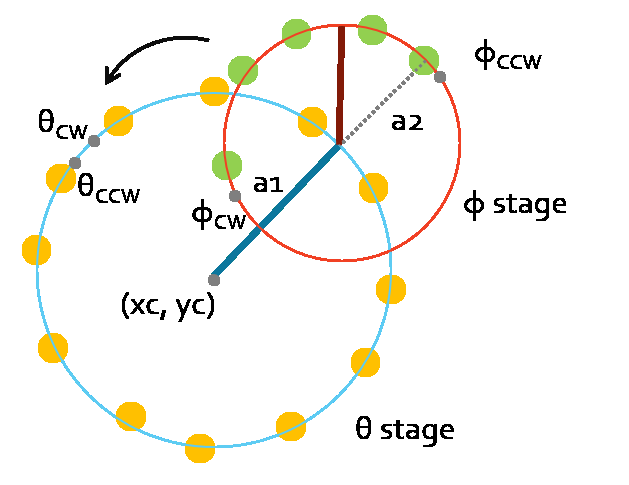
\includegraphics[width=75mm]{Calib_D3.eps}
\end{center}
\caption{Schematic picture of Cobra parameters.
Orange and green spots imply the positions of blinking fiber in F3C.
Light-blue and red circles indicate fitted circles for fiber spots.
}
\label{fig:Cobraparams}
\end{figure}


\begin{itembox}[l]{\suctitle{Success Criteria}}
The brightness of back-lit fibers are regulated. \\
Parameters of each Cobra $(x_{c,k}, y_{c,k}, a_{1,k}, a_{2,k}, \bm{\theta _{0,k}}, \bm{\theta _{m,k}}, \bm{\phi _{0,k}}, \bm{\phi _{m,k}})$ are measured and stored to MPS.

\bluetext{Required long time to analyze the data?: No. \\
--- We shall analyze the data in real-time.
In addition, cobra parameters will be stored in short time scale.
}
\end{itembox}
%%%%%%%%%%%%%%%%%%%%%%%%%%%%%%%%%%%%%%%%%%%%
\subsubsection{Characterization of PSF and Spectral Distribution [Daytime/Nighttime]}\label{secflow:PSFchar}

\milestone{The light is delivered from the primary mirror to the detectors for the first time.}

In this step, we measure PSFs and the spectral distribution on the detectors.
As twist of fiber changes, PSF depends on telescope positions as well as Cobra position in its patrol area.
This step is similar to step \ref{secflow:SpSchar}, but the data includes all optics and systems; namely, Primary Mirror --- WFC, --- Field Element --- Cable C --- Cable B --- Cable A --- SpS, and all connectors between them.

PSF/spectral distribution image will be sent to 2D DRP team of Princeton University, who will characterize them in detail.
We will check basic properties of PSFs such as FWHM etc., though.

This sequence consist of three step: (1) principal characterization, (2) measurement of sky spectra, and (3) characterization according to Cobra movement.
The arc/flat lamp on PFI is used to measure PSFs/spectral distribution of all fibers.
We therefore also check the uniformity of the calibration lamps, and validate the calibration sequence.

\paragraph{Principal Characterization}
As soon as PFS can deliver light from the primary mirror to the Spectrograph detector, we will take arc and flat.
As of the writing (June 2016), it can be done during PFI check on Telescope (\ref{secflow:PFIon}), because PFI, Cable B and two SMs will be delivered.
In order to look into the PSF, we shall dithered flat as well.
Dark and bias data is needed for calibration.
Check wavelength resolution, wavelength coverage for all fibers.

Once Cobra calibration is carried out, sparse arc and flat shall be taken in order to look into the PSF wing.
How sparse is TBD, but we can estimate AIT data at LAM.
Current plan\footnote{In his draft, he requested to observe semi-crowded fields before we can target objects for demonstration and PR. May be it can be done during later phase of \ref{secflow:1stDM}, if it is acceptable accurate fiber positioning is crucial.} by Robert Lupton from Princeton University (2D-DRP team) is every other fibers and every 10th fibers with shorter and longer integrations.

\paragraph{Measurement of Sky Spectra}
We will take arc and continuum image with changing telescope elevation and/or RoA.
For example,
\begin{itemize}
\item RoA = $-270, -180, -90, -60, 0, +60, +90, +180, +270$ (9 positions)
\item Elevation = $30, 45, 60, 75$ (4 positions)
\end{itemize}
%If we hide every 3 fibers on the detector with the dots, we need 3 types of fiber configuration.
If we take 3 types fiber configuration (e.g. full, a little sparse, very sparse), there are $3 \times 4 \times 9 = 108$ configurations in total.
%Therefore, there are $4 \times 9 = 108$ configurations in total.
Assuming that it takes 5 minutes to configure, and acquire a couple of images, it will take 9 hours for a series of either arc or continuum images.
As time will be limited, we will firstly characterize PSFs in operation RoAs at every elevation angles, and then study other RoAs.
If we take images at 9 RoA positions at El=60 degree, and 3 RoA operational positions at other elevations (18 telescope positions in total), it will take 4.5 hours.
In the current plan, required time is estimated assuming measurement at 18 positions.
Ideally, as sky condition changes during a night, we shall revisit to a given elevation and RoA every hour or so.

By comparing the properties of PSF such as FWHM, we examine dependency and repeatability of the spots on telescope pointing.
%It is difficult to take arc/continuum image using calibration lamps with telescope pointing to other direction than zenith.
%We will use sky as light source for PSF measurement.
%At this moment, it is not necessary to moving fiber positioner, because we can take spectra of somewhere of the sky.
In the PFS operation RoA is limited from $-60 \deg$ to $+60 \deg$, considering that impact of twisted fibers on FRD.
During the commissioning, however, we shall check the PSFs in wider range of RoA.
If the impact is enough low at wider RoA, we can have more flexibility of operation (e.g. constraint due to dots.).

\paragraph{Characterization according to Cobra Movement}
In this sequence, we also examine PSF variance with respect to the Cobra rotation angles ($\theta$, $\phi$).
Here, we use calibration lamps with the telescope pointing at zenith.
If we change Cobra positions by 60 degrees, namely
\begin{itemize}
\item $\theta$ = $0, +60, +120, +180, +240, +300, +360$ ($0, +360$ mean limit angles)
\item $\phi$ = $0, +60, +120, +180$ ($0, +180$ mean limit angles)
\end{itemize}
We will take $3 \times 7 \times 4 = 84$ sets of data, for 3 fiber configurations.
We will take $3 \times 7 \times 4 = 84$ sets of data, for 3 fiber configurations.
It will take 7 hours to acquire a series of arc data.
We shall take images while Cobras are moving.

\bigskip

During the commissioning phase, SMs 1, 2, and 3 will be delivered ahead of the delivery of PFI.
Therefore, we can repeat the same test for the first three SMs when SM4 will be tested.
Alternatively, if we can characterize PSF well for the first SMs, we can limit the PSF test for the last SM, in order to minimize the telescope time.

In either case, the test using sky shall be limited, for example
\begin{itemize}
\item RoA = $-60, 0, +60$ (3 positions)
\item Elevation = $30, 60$ (2 positions)
\end{itemize}
In this case, it will take 0.5 hours for either arc or continuum data.

%\redtext{Measure wavelength resolution, wavelength coverage. 
%Sequence \ref{secflow:PSFchar} can be skipped at least wavelength resolution and coverage for SM3,4, which will be ready in August 2018.}

\paragraph{Designated Tool fot This Process}
Detailed analysis will be done by 2D-DRP team (Princeton).
For PFS commissioning, a tool for measure FWHM is needed.

\begin{itembox}[l]{\suctitle{Success Criteria}}
The dependency of PSF and spectral distribution on Telescope elevation and RoA is measured.

\bluetext{Required long time to analyze the data?: No. \\
--- Detailed PSF characterization is mainly carried out by 2D-DRP team, and we will proceed to the next sequence in parallel with analysis.
}
\end{itembox}
%-- replaced to each other: 25 Apr. 2016 : end
%%%%%%%%%%%%%%%%%%%%%%%%%%%%%%%%%%%%%%%%%%%%%
\subsubsection{Calibration of the Distance b/w A\&G Cameras and the Fixed Fiducial Fibers [Night-time]}\label{secflow:agc2fff}

In this step, we calibrate the position of the A\&G cameras relative to their fixed fiducial fibers, in order to make the sky-PFI relation  consistent between A\&G cameras and the field of view.

Firstly, we slew the telescope to have a star in the center of an A\&G camera.
Then we move the telescope to have the AG fixed fiducial fiber pointed to the star.
We execute the raster scan around the fixed fiducial fiber and calibrate the distance between A\&G camera and the fiber.
Because one A\&G camera has two fiducial fibers on both sides in the azimuth direction, the raster scan should be carried out using both fibers.
Therefore, we shall do $12 \times n$ raster scan in total.

Using the calibrated data, the transformation from Sky Catalogue ti F3C is updated.

\begin{itembox}[l]{\suctitle{Success Criteria}}
Calibration of the distance between the AGC and the AG fiducial fibres is succeeded.
\end{itembox}
%%%%%%%%%%%%%%%%%%%%%%%%%%%%%%%%%%%%%%%%%%%%
\subsubsection{Second-Pass Distortion Map [Night-time]}\label{secflow:raster}

After the process \ref{secflow:1stDM}, the science fibers should be pointed to the targets with the accuracy of $\sim 50$ um (at least less than 100 um).
In this step, we will do raster scan to improve the distortion map and achieve the fiber pointing accuracy of $\sim 10$ um RMS.

The process is as follows:
\begin{enumerate}
\item Slew the telescope to the field where enough bright stars is cataloged with good astrometry (see section \ref{sec:RasterField}).
\item Put these bright stars on the science fibers and take fiber spectra with the telescope moving in 3$''$ $\times$ 3$''$ grid, approximately three time as large as the fiber core diameters.
Note that the raster with 5 position of hexagonal pattern provide denser scan than the grid (TBD).
\item Calculate the brightest position by comparing the intensity of these spectra.
\item Repeat 1.--3. for several fields at various telescope positions, and calibrate the distortion map.
\item Check the dependency of the map on wavelength, and check if ADC works correctly, by comparing the observed positions with predicted ones by ADC.
\end{enumerate}
Calibrations will include the following factors:
\begin{itemize}
\item Telescope elevation, and azimuth
\item Temperature
\item Focus
\item ROA
\item Error in the relative position of A\&G cameras to fiber positioner.
\item Error in Cobras' position measured prior to integration at Subaru
\item Error in Catalogue
\item ADC
\item etc…… (TBD)
\end{itemize}

Assuming we take 120- --150-second exposure for a given position, it will take $\sim$ 30 minutes including slewing and fiber configuration.
We will take 2 sets of 4 El $\times$ 4 RoA positions ($\sim$ 8 hours) to study the dependence of the above parameters.
We repeat 2 times of these sets using SMs 1--3 (runs. 4 and 5).
Note that fibers of each SM are arranged on the focal plane to cover entire field of view, we can study distortion without SM4.
However, we will check and finalize the distortion map using all SMs at run 6.
In total, 5 nights are required in this process.

When the second distortion map is made, update ETS using this map, and/or update the repository for coordinate transformation (TBC).

\paragraph{Designated Tool for This Process}
A tool for measuring the brightest position from raster scan data.

\begin{itembox}[l]{\suctitle{Success Criteria}}
Second distortion map is obtained with error less than 10um.

\bluetext{Required long time to analyze the data?: Yes. \\
--- It takes time ($\sim$ one month) to improve distortion map, by analyzing raster scan data in various condition.
Also it needed more than one run to check dependency of temperature and so on.
}
\end{itembox}

When this step is completed, the fibers shall point to the target within the accuracy of 10 um.
Then, we verify the instrument performance in the following steps. 
%%%%%%%%%%%%%%%%%%%%%%%%%%%%%%%%%%%%%%%%%%%%
\subsubsection{Performance Verification I [Night-time]}\label{secflow:PV1}

\milestone{We operate full observation sequence for 900-sec exposure for the first time.}

\milestone{PFS acquire faint galaxies/stars spectra for the first time.}

The goal of this commissioning stage is to verify the performance of the integrated PFS system. 
Specifically, after we confirm that the observational sequence in order to carry out scientific observations can be made, we measure the total throughput from end to end, i.e., from the primary mirror of the telescope to the detectors, with actual celestial objects. 

\begin{itemize}

\item{Verification of the observation sequence}

The following points, which correspond to the sequence itself that is supposed to be carried out in normal science observations, will be verified:

\begin{enumerate}
\item{Acquisition of the target field}
\item{Confirmation of the guiding}
\item{The cobra configuration for target objects}
\item{Start exposure}
\item{Acquisition of the next target, if any}
\end{enumerate}

At this sequence, we test that all commands can be sent correctly.
We have requirements for overheads, assuming typical exposure time of 900 seconds.
According to {\tt REQ-SYS-520 (Test)}, the taken time from field acquisition to starting auto guiding is within 105 seconds, which this shall be confirmed in \ref{secflow:AGCfunc}.
By selecting a field where all science fibers should be allocated objects, we test whether 95 \% of 2394 fibers (2275 fibers) moves to the their targets within 105 seconds {\tt REQ-SYS-517 (Test)}, with accuracy of $<$ 10um. 
We shall take 900-sec exposure, during which the tracking error should be $\sim$ 0.2 arcsec rms by auto guiding (0.2 arcsec rms for 10 minites and 0.6 arcsec rms for 30 minites: {\tt REQ-SYS-888 (Test)}).
(It seems the first time to track a field for longer period, $>$ 10 minutes, because we execute short exposures in the previous sequences.)
After exposure, it should take less than 35 seconds to readout detectors, archive the fits (including MCS data for finally configured fiber image) data and telemetry data to STARS, Subaru archiving system ({\tt REQ-SYS-519}). 


\begin{itembox}[l]{\suctitle{Success Criteria}}
Confirm that the normal observation sequence can be carried out.
\begin{itemize}
\item 95 \% of science fibers can be allocated to their objects within 105 seconds, and allocation error should be less than 10 um. 
\item Tracking error for 10 minutes and 30 minutes is 0.2 arcsec rms and 0.6 arcsec rms. 
\item Reading out the detectors and archiving data are completed for less than 35 seconds. 
\end{itemize}
\end{itembox}

\item{Measurement of the total throughput}

The throughput is estimated using measured transmissions / reflection curve for each optical components (e.g. the primary mirror, fibers, optics for Spectrographs).
The expected PFS performance is shown on the web.\\
\hspace*{10mm} http://pfs.ipmu.jp/research/performance.html \\
In this test, we measure the throughput of the entire system and compare with the prediction.

The process of the total throughput measure will be carried out as the following way:

\begin{enumerate}
\item{Observe stars with known spectral types}

This process requires a substantial number of stars whose spectral types and absolute flux are known. The spectra should have as less spectral feature in the observed wavelength range as possible, therefore F-type dwarf stars will be a suitable candidate for this measurement. The number of stars in the observations should be ideally equal to the number of fibers per one FoV. Star clusters will be a good candidates.

\item{Comparison of the observed counts to the given flux density as a function of wavelength}

We will compare the obtained spectra to the given spectra of the observed stars. From the given spectra, the expected counts as a function of wavelength can be calculated by assuming atmospheric transmission. By comparing the obtained counts and expected counts, the total throughput can be estimated.

\item{Repeat this measurement and comparison in various conditions}

The total throughput measurement should be carried out in different conditions (e.g., weather including different seeing, cobra configuration, telescope EL, and ROA, etc.). The average value will be the representative measured value of the total throughput. 

\item{Comparison of the obtained throughput to the expected one}

If the measured value is significantly different from the expected total throughput, we might need to verify the input source. In FMOS engineering observations, they checked the total throughput measurement with celestial objects by using a black body furnace. In this case, the optimization of the set up of the blackbody furnace, such as position, incident angle, and the calibration of absolute flux, would need to be considered.

\end{enumerate}

The time duration of this commissioning stage will be about 1 engineering run, i.e., about 2--3 engineering nights, taking into consideration of a weather factor.

\begin{itembox}[l]{\suctitle{Success Criteria}}
Confirm that the total throughput of PFS is as expected:\\
BLUE arm --- $\sim$12\% (380--450 nm), $\sim$21\% (450--550 nm) and $\sim$24\% (550--650 nm) \\
RED arm (LR) --- $\sim$30\% (630--750 nm), $\sim$29\% (750--850 nm) and $\sim$27\% (850--970 nm) \\
RED arm (MR) --- $\sim$26\% (710--875 nm), $\sim$28\% (775--825 nm) and $\sim$27\% (725--885 nm) \\
NIR arm --- $\sim$17\% (940--1050 nm), $\sim$19\% (1050--1150 nm), and $\sim$17\% (1150--1260 nm)
\end{itembox}

\end{itemize}
\begin{itemize}
\item{Verification of the absolute flux calibration}

One of the important tasks is the establishment of the absolute flux calibration process. In the normal observations of faint objects such as distant galaxies, we suppose that a certain fraction of fibers is used for flux calibration stars, for which F-type stars are desirable. By using the flux calibration stars, the spectra of all other fibers will be calibrated. In this measurement, we verify whether the absolute flux calibration process can be made at the expected level, with the accuracy of 5 \% ({\tt REQ-SYS-656 (Test)}). The measurement process will be done as follows:

\begin{enumerate}
\item{The process is closely related to the measurement of the total throughput described in the previous subsection. In this measurement, we observe a substantial number of stars whose spectral types and absolute flux are known, including flux calibration stars. The data reduction is done following the normal procedure.}

\item{The calibrated spectra can be compared to the given spectra. The deviation from the expected spectra can be calculated as a function of wavelength. If necessary, this measurement will be done in various different condition such as ones listed in the previous subsection, and the deviation of the flux calibration as a function of these quantities.}

\item{The cross-correlation to the external catalogue will be useful especially for faint galaxies. In this measurements, targets selected from the external catalogue (e.g., SDSS) will be observed and the data processing will be done in the normal procedure. We check the obtained spectra and the deviation from the external SDSS spectra.}

\item{Verify the following items:}
\begin{itemize}
\item{that absolute flux calibration can be done at the desired level of accuracy (5 \%)}
\item{the number of objects that should be used for the calibration}
\item{the spectral type of stars that is optimal and acceptable for the desired flux calibration}
\item{the optimal spatial distribution of the calibration stars on the FoV}
\end{itemize}
\end{enumerate}

\begin{itembox}[l]{\suctitle{Success Criteria}}
Confirm that the absolute flux calibration can be done with the accuracy of 5 \%. \\
The number of fibers for flux calibration is determined (100--200 ? TBC).
\end{itembox}

\item{Verification of sky background subtraction}

The subtraction of the sky background in the data analysis is one of the most critical tasks in the PFS projects. 
In this verification process, we allocate all fibers on the sky, among which we choose some of them as the sky fibers.
Then we test sky subtraction by checking the reduced data of the rest fibers, selected as ``scientific object".
If the sky background is subtracted perfectly, the reduced spectra should be ``flat". 
We also observe a substantial number of faint objects that is supposed to be observed in the actual scientific operations. In the normal and expected observations, a certain fraction of total fibers will be used for the sky background subtraction. We will estimate the residual of the sky subtraction as a function of:
\begin{enumerate}
\item{exposure or observing time}
\item{airmass}
\item{other weather condition such as seeing}
\item{cobra configuration and ROA?}
\end{enumerate}

We verify whether the sub subtraction residual is in the range of the expected level (0.5 \% accuracy{\tt REQ-SYS-679 (Analysis)}) or not. 
Another important items to be verified is the number of the sky fibers that is required for the desired sky subtraction.

\begin{itembox}[l]{\suctitle{Success Criteria}}
Confirm that the sky background can be subtracted within the accuracy of 0.5 \%.
\end{itembox}

\item{Verification of the limit of exposure time in each frame}

According to {\tt REQ-SYS-732 (Demonstration)}, the exposure time for one frame shall range 10 sec -- 1800 sec. 
The maximum exposure time is determined not to have too many cosmic rays, nor saturated sky emission lines.
In this verification process, we will determine the maximum exposure time for one frame by taking a substantial number of frames with longer exposure ($>$ 150 sec. TBC). 
The purpose of this verification is as follows:

\begin{itemize}
\item{Check the fiber loss as a function of time}
\item{Effects on the sky subtraction}
\item{Check the saturation of OH emission lines}
\item{Effects by cosmic ray on obtained spectra and data reduction process}
\item{Check the instrument stability (c.f. FMOS instability problem during engineering observation)}
\end{itemize}

\begin{itembox}[l]{\suctitle{Success Criteria}}
Confirm that the maximum limit of long exposure time ($<$ 1800 sec) in each frame can be verified.
\end{itembox}

\item{Verification of observations with a long total exposure time}

In the observations targeting very faint objects such as high-redshift galaxies, very long exposure time in total will be supposed. The signal-to-noise ratio of the obtained spectra should, ideally, increase with exposure time just as expected. In this verification process, we will carried out observations with very long exposure time in total ($\sim$10-20 hours). The target is supposed to be both bright and faint galaxies. In the measurement, we will check the following points:

\begin{itemize}
\item{The obtained signal-to-noise ratio grows as a function of exposure time following $\propto \sqrt{t_{exp}}$.} 
\item{The effect of very long exposure on the sky subtraction.}
\end{itemize}

The time duration of this commissioning stage will be about 2 engineering runs, i.e., about 5--7 engineering nights, taking into consideration of a weather factor.

\begin{itembox}[l]{\suctitle{Success Criteria}}
Confirm that the expected growth of Signal-to-Noise ratio of faint targets for long exposure time
\end{itembox}

\item{Verification of re-configuration of cobra during scientific observations}

\begin{itembox}[l]{\suctitle{Success Criteria}}
Confirm weather the re-configuration of cobra during observations with long total exposure time and how often the re-configuration is needed
\end{itembox}

\item{Verification of beam-switching mode (TBD)}

\end{itemize}

%%%%%%%%%%%%%%%%%%%%%%%%%%%%%%%%%%%%%%%%%%%%
\subsubsection{Performance Verification II [Night-time]}\label{secflow:PV2}

In the previous commissioning process (\ref{secflow:PV1}), basic instrument parameters and performance will be revealed. After this phase, a normal observational sequence can be done properly using almost the same software interface used in actual survey observations including data reduction pipeline. 

In this this commissioning phase, we will stabilize the instrument operation and the performance optimizing the softwares and the operation processes for long-term survey observations. Specifically, we will conduct the following verifications:

\begin{itemize}
\item Long exposure of faint galaxies and stars
\item DRP optimization using a wide variety of galaxies and stars 
\item Confirmation that there is no time change of the performance
\end{itemize}



\begin{itembox}[l]{\suctitle{Success Criteria}}
\begin{itemize}
\item Confirm that observation process can be done properly and stably
\item Confirm that there is no time change of the instrument performance
\item Confirm that a sufficient number of galaxies and stars was observed to optimize the 1D-DRP using a machine learning technique
\end{itemize}
\end{itembox}




% Raster Fields
%%%%%%%%%%%%%%%%%%%%%%%%%%%%%%%%%%%%%%%%%%%%
\section{Selection of Observing Fields [TBD]\label{sec:RasterField}}

In this section, we describe the preparation of target objects for the on-sky commissioning and the performance verification. We suppose three cases of target fields, 1. a field with many bright stars such as an open cluster for the raster scan, 2. a field with a sufficient number of bright stars such as an SDSS field at high galactic latitude for the throughput measurement and the verification of the flux calibration, 3. a field with faint galaxies and stars for the verification of long exposure. We briefly describe each case and possible candidate targets below.

\subsection{Open Clusters as the Raster Targets}
For the raster scan process, targets should be sufficiently bright and point sources for the accurate evaluation in the analysis. In addition, they should cover the entire PFS FoV and the number density should be matched to the PFS fiber density. Open clusters with sufficient bright member stars in the Galaxy are plausible targets for the raster scan. 

The candidate open clusters are selected from DAML02 catalogue (Dias et al. 2002, A\&A, 389, 871), which includes information on fundamental parameters (distance, apparent diameter, proper motion, age, reddening, metallicity, and so on) of $\sim2000$ open clusters.  Figure \ref{fig:RasterFieldMap1} and Figure \ref{fig:RasterFieldMap2} show the spatial distribution of the open clusters with the apparent diameter ($d$ [deg.]) of $>30$. There exist $\sim130$, $\sim50$, $\sim30$ open clusters with the apparent diameter of $30<d<60$, $60<d<120$, and $d>120$, respectively. The typical number of member stars is $\sim1000$. 

\begin{figure}[!ht]
\begin{center}
\includegraphics[width=150mm]{map_ucac4_openclusters_combined_f160.pdf}
\end{center}
\caption{Stellar density with objects $f<16.0$ mag taken from UCAC4 catalog in color map (left) and contour (right). The spatial distribution of open clusters with the apparent diameter ($d$ [deg.]) of $d>30$. from DAML02 catalogue is also plotted in both panels. Open clusters with $30<d<60$, $60<d<120$, and $d>120$ are shown by \textit{blue}, \textit{green}, and \textit{red circles}, respectively. The size of symbols represents the number of member stars.
}
\label{fig:RasterFieldMap1}
\end{figure}

\begin{figure}[!ht]
\begin{center}
\includegraphics[width=150mm]{map_ucac4_openclusters_combined_f160_gc.pdf}
\end{center}
\caption{Similar to Figure \ref{fig:RasterFieldMap1}, but on the Galactic longitude and latitude.
}
\label{fig:RasterFieldMap2}
\end{figure}


\begin{table}[!ht]
\begin{center}
\caption{}
\label{tab:open_clusters}
\begin{tabular}{lccccc}  \hline
Name &  R.A. & Dec. & Diameter & \# of members & Mag. limit\\ 
          & [hh:mm:ss] & [dd:mm:ss] & [arcmin] & & [mag]\\
\hline \hline
Collinder 464 & 05:12:39 & +73:58:29  & 120.0 &  5212 & TBC  \\
Melotte 31     & 05:18:10 & +33:22:25  & 135.0  & 14341 & TBC \\
Melotte 111   & 12:25:06  & +26:06:00 & 120.0   & 863 & TBC    \\         
Collinder 471 & 22:07:06  & +72:00:00 & 130.0  & 4573 & TBC \\
\hline
ASCC 19       & 05:27:47 & $-$01:58:48  &  96.0    &  2412 & TBC \\
Collinder 89   & 06:18:00 & +23:38:00  &  60.0    &  2971 & TBC \\
Alessi 33        & 07:01:59 & $-$26:30:12  &  60.0   &   3371 & TBC \\
IC 2944$^{*}$  & 11:38:20  & $-$63:22:22  &  65.0   &  8860 & TBC \\
Trumpler 24$^{*}$  & 16:57:00  & $-$40:40:00 &  60.0   &  5720 & TBC \\
ASCC 88$^{*}$    & 17:06:47  & $-$35:36:00  &  66.0  &  6501 & TBC \\
ASCC 111       &  20:11:13 & +37:27:00 &  66.0  &  8004 & TBC \\
ASCC 125      &  22:56:17 & +62:45:00  &  66.0  &  2332 & TBC \\
\hline \hline
\end{tabular}
\end{center}
*: These targets cannot be observed with a good visibility.
\end{table}


\subsection{Field Bright Stars}
As Figure \ref{fig:RasterFieldMap1} and Figure \ref{fig:RasterFieldMap2} show, the spatial location of the available open clusters with sufficient apparent diameter for the PFS FoV is very limited. We thus consider the possibility of using normal field stars as raster scan targets in this subsection. In Figure \ref{fig:RasterFieldMap1} and Figure \ref{fig:RasterFieldMap2}, the density map of stars with $f<16.0$ mag. selected from the UCAC4 catalogue (Zacharias et al. 2013, AJ, 145, 44), which contains 113 million stars down to $R\sim16$ mag for which the positions determined with the accuracy of $<100$ mas. Although the number of available stars in one PFS FoV is limited in the high galactic latitude ($b$), there exist sufficient available stars of f$<16$ mag in $b<60$ deg.

\subsection{Faint Galaxies and Stars}
Basically, faint targets to verify the system performance will be selected from objects detected with HSC imaging data, which are candidate targets in the actual large survey with PFS. 


\subsection{Detailed Procedure of Raster Scan}
TBW

\subsection{List of Candidate Raster Fields}
TBW

\begin{figure}[!ht]
\begin{center}
\includegraphics[width=150mm]{map_sdss_r16-17_colm_combined_20151208.pdf}
\end{center}
\caption{Stellar density with objects $r<16.0$ mag (left) and $r<17.0$ mag taken from SDSS DR12 catalog in color map. 
}
\label{fig:RasterFieldMapSDSS1}
\end{figure}

\begin{figure}[!ht]
\begin{center}
\includegraphics[width=150mm]{map_sdss_r16-17_colm_gc_combined_20151208.pdf}
\end{center}
\caption{Similar to Figure \ref{fig:RasterFieldMapSDSS1}, but on the Galactic longitude and latitude.
}
\label{fig:RasterFieldMapSDSS2}
\end{figure}


% Coordinates systems
%%%%%%%%%%%%%%%%%%%%%%%%%%%%%%%%%%%%%%%%%%%%
\section{PFS Coordinates and Calibrations in Commissioning Procedure}

\subsection{Definitions of Coordinates}
PFS has four coordinates used for fiber positioning: Sky Catalogue, Fixed Fiducial Fiber Coordinate (F3C), Cobra Coordinate, and Meteorology Camera System Coordinate (MCSC).

The definitions of each coordinates are as follows.

\paragraph{Sky Catalogue}
The sky targets such as galaxies and stars as well as sky backgrounds lie on this coordinates.
We describe the target positions using the equatorial coordinates $\bm{S}=(\alpha , \delta)$ in the unit of degree.
In the operation, we slew the telescope to a given field centered at $\bm{S}=(\alpha [ \degree ], \delta [ \degree ])$.
In this Field of View, the sky targets have a position on Sky Catalogue as the differential from the center: $\bm{S_k}=(\Delta \alpha _k [ \degree ], \Delta \delta _k [ \degree ])$.

\paragraph{Fixed Fiducial Fiber Coordinate (F3C)}
In order to calculate fiber positions at each exposures, 97 fixed fiducial fibers are used.
F3C is the coordinate from the viewpoint of these fibers.
In this coordinate, sky targets and fiber positions are described in the unit of mm: $\bm{X_k}=(x_k [ \mathrm{mm} ], y_k [ \mathrm{mm} ])$.
In practical, F3C is roughly defined as  mean plane of the top surface of the fixed fiducial fibers.
F3C resembles physical metrics of PFI (Prime Focal Instrument), but in fact it is {\it different} because the orientation between each fiducial fiber is constant in F3C.
For example, consider the case where the Focal Plane expands along with the increase of the temperature.
In such a case, the separation of the two fiducial fibers gets larger, whilst the separation in F3C doesn't change at all (see Figure \ref{fig:F3Cex1}).
% no distortion, no thermal expansion etc.

\begin{figure}[!ht]
\begin{center}
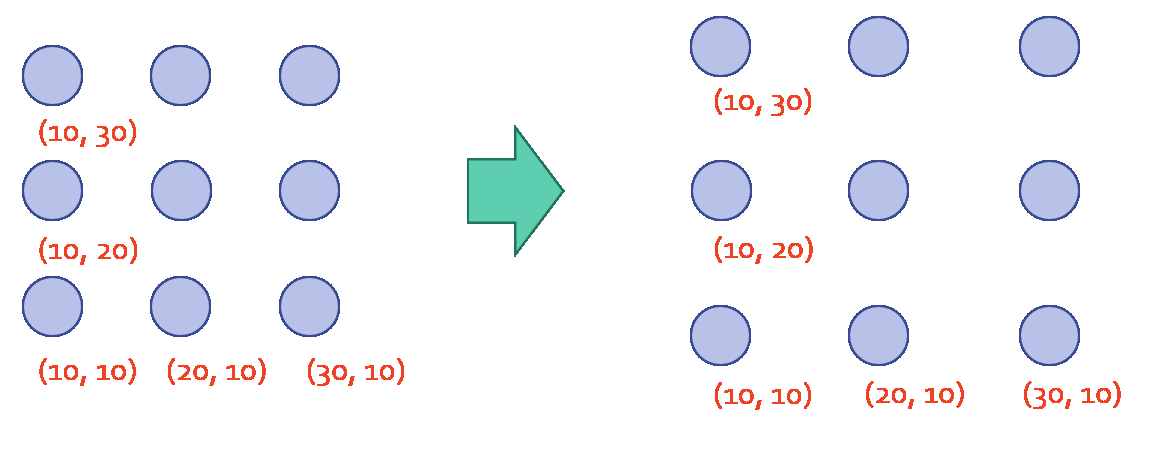
\includegraphics[width=100mm]{F3C_example1.eps}
\end{center}
\caption{An example of the change in physical metrics of fiducial fibers (blue circles).
The fiber positions in F3C are described in red letters.
}
\label{fig:F3Cex1}
\end{figure}

Another example explaining the difference between F3C and the physical metrics of PFI is the case where one of the fixed fiducial fibers happens to shift from the original position (Figure \ref{fig:F3Cex2}).
In such case, the positions of all fixed fiducial fibers are constant again.
Measure for this case is described in section \ref{sec:failures}.

\begin{figure}[!ht]
\begin{center}
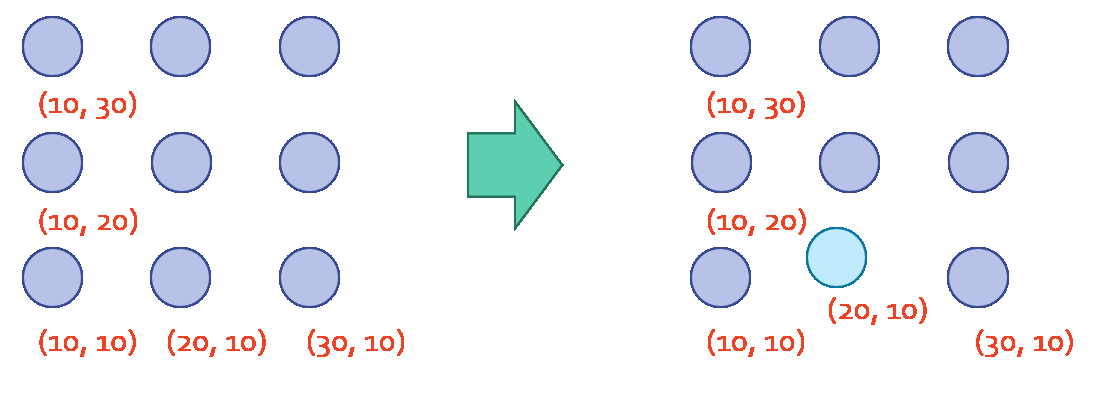
\includegraphics[width=100mm]{F3C_example2.eps}
\end{center}
\caption{Another example of the change in physical positions of fiducial fibers (blue and light-blue circles).
The fiber positions in F3C is described in red letters.
}
\label{fig:F3Cex2}
\end{figure}

\paragraph{Cobra Coordinates}
The fiber positioner ``cobra" is a two-axis motor; $\theta$ stage and $\phi$ stage.
The motion of each cobra is controlled by MPS (Movement Planning Software) with the two angles of these stage in degree.
We call the two angle as the Cobra Coordinates: $\bm{C_k}=(\theta _k [ \degree ], \phi _k [ \degree ])\;, [k=1,2,....,2394]$ .

\paragraph{Meteorology Camera System Coordinate (MCSC)}
The subsystem Meteorology Camera System calculates centroids of back-illuminated fibers.
Here, the centroids are determined as the position on CMOS sensor in the unit of pixels, equivalent to MCSC.
The centroids of the fibers, therefore, is determined in MCSC as $\bm{F_k}=(i_k [ \mathrm{pixel} ], j_k [ \mathrm{pixel} ])$.

\subsection{Observational Sequence and Definitions of Coordinate Transformations}\label{sec:ctsec}

\begin{figure}[!ht]
\begin{center}
\includegraphics[width=150mm]{ObservationalSequence.eps}
\end{center}
\caption{PFS observational sequence and coordinates transformations.
}
\label{fig:obssec}
\end{figure}

Figure \ref{fig:obssec} shows observational sequence in particular during positioning fibers, and transformations of the above coordinates.
The procedure of fiber positioning is as follows:
\begin{enumerate}
%%% 1. sky
\item ETS (Exposure Time Sequencer) calculate the target positions $\bm{S_k}=(\Delta \alpha _k [ \degree ], \Delta \delta _k [ \degree ])$ in the observed field centered at $\bm{S}=(\alpha [ \degree ], \delta [ \degree ])$.
%%% 2. sky -> F3C
\item ETS transforms the target positions in Sky Catalogue to those in F3C using the telescope parameters at that moment ($Az, El, InR, T$).
We define this transformation as $D_1$.
That is,
\begin{equation}
\begin{array}{crcl}
& \bm{S_k}=(\alpha _k [ \degree ], \delta _k [ \degree ]) & \rightarrow & \bm{X_k}=(x_k [ \mathrm{mm} ], y_k [ \mathrm{mm} ]), \\
& & D_1 & \\
\mathrm{or} & \bm{X_k} &= & D_1(\bm{S_k}).
\end{array}
\end{equation}
In practical, firstly ETS calculates ($Az, El, InR$) at a given time for the filed centered at $\bm{S}$, or receives them from the telescope.
Then ETS calculates ($\Delta Az [ \degree ], \Delta El [ \degree ]$) of each target $\bm{S_k}$, as the offset of the field center.
This offset is transformed to the position on F3C using $D_1$.
That is,
\begin{equation}
\begin{array}{rcccl}
\bm{S_k}=(\alpha _k [ \degree ], \delta _k [ \degree ]) & \rightarrow & (\Delta Az [ \degree ], \Delta El [ \degree ]) & \rightarrow & \bm{X_k}=(x_k [ \mathrm{mm} ], y_k [ \mathrm{mm} ]), \\
& & & D_1 & \\
\end{array}
\end{equation}
%%% 3, MCSC -> F3C
\item\label{item:mcs2f3c} Take fiber image with MCS and measure fiber positions $\bm{F_k}=(i_k [ \mathrm{pixel} ], j_k [ \mathrm{pixel} ])$.
Then FPS (Fiber Positioning Sequencer) transforms the fiber positions in MCSC to those in F3C.
We define this transform as $D_2$.
That is,
\begin{equation}
\begin{array}{crcl}
& \bm{F_k}=(i_k [ \mathrm{pixel} ], j_k [ \mathrm{pixel} ]) & \rightarrow & \bm{X'_k}=(x'_k [ \mathrm{mm} ], y'_k [ \mathrm{mm} ]), \\
& & D_2 & \\
\mathrm{or} & \bm{X'_k} & = & D_2(\bm{F_k}).
\end{array}
\end{equation}
%%% 4. F3C -> MPS
\item\label{item:f3c2cobra} MPS calculates Cobra Coordinates to be commanded, by comparing the position of fibers $\bm{X'_k}$ and targets $\bm{X_k}$.
We call this transformation $D_3$.
\begin{equation}
\begin{array}{crcl}
& \bm{X_k}=(x_k [ \mathrm{mm} ], y_k [ \mathrm{mm} ]), \bm{X'_k}=(x'_k [ \mathrm{mm} ], y'_k [ \mathrm{mm} ]) & \rightarrow & \bm{C_k}=(\theta _k [ \degree ], \phi _k [ \degree ]) ,\\
& & D_3 & \\
\mathrm{or} & \bm{C_k} & = & D_3(\bm{X_k},\bm{X'_k}).
\end{array}
\end{equation}
%Comparing these positions, MPS derives the angles to move cobras $\bm{C_k}$:
%\begin{equation}
%\begin{array}{crcl}
% & \bm{C_k} & = & D_3(\bm{X'_k}) - D_3(\bm{X_k}).
%\end{array}
%\end{equation}
Then move Cobras following the derived angles $\bm{C_k}$.
%%% 5. repeat
\item Repeat \ref{item:mcs2f3c} and \ref{item:f3c2cobra} until the differential between the target and the fiber positions meets the required accuracy; $\Delta r_k= \sqrt{ \Delta x_k^2 + \Delta y_k^2} \leq 10 \;\mathrm{[um]}$ (TBC; {\tt REQ-SYS-553}).
FPS judges which fibers should be moved, and sends $\bm{X_k}$ and $\bm{X'_k}$ to MPS.
\end{enumerate} 

Formation of $D_1$ and $D_2$ is determined by the Project Office and stored to a designated repository (TBC), while $D_3$ is determined by JPL.
During the commissioning, the transformation functions $D_1$, $D_2$, and defined and/or calibrated, and calibration for $D_3$ are executed.
In the following section, these process are described.

%------------------------------
% subsection: calibrations
%------------------------------
\subsection{Calibrations of Coordinate Transformation during the Commissioning}\label{sec:coord_calib}

Before shipping to the Subaru, the physical positions of all fixed fiducial fibers, science fibers and A\&G Cameras are measured at a given temperature during the integration of PFI in Taiwan.
We shall use the positions of fixed fiducial fibers at that time as their coordinates in F3C.

\paragraph{Sky Catalogue to F3C transformation $D_1$:}
%In order to transform target coordinates in Sky Catalogue to those in F3C, we use the HSC distortion map $D'_{1,0}$ as the first step.
In order to transform target coordinates in Sky Catalogue to those in F3C, we use the WFC as-built model $D'_{1,0}$ as the first step.
Using this model, the position on PFI is calculated by Yoko Tanaka from Subaru telescope.
We call this distortion map ``$0^{th}$-pass distortion map".
The detail of the ``$0^{th}$-pass distortion map" is under development.
%As of the time of writing, ``$0^{th}$-pass distortion map" is described in the form of 9-order Polynomial of x and y \footnote{According to the HSC DRP team (Pfof. Robert Lupton), the 9-order polynomial is not suitable in particular to the edge of FoV. The PFS FoV including A\&G Cameras ($\sim 0.71 \degree$), however, seems smaller enough to use the same function as ``$0^{th}$-pass distortion map". They will improve the form in the future.}.
%As of the time of writing, ``$0^{th}$-pass distortion map" is described in the form of $9^{th}$-order Chebyshev polynomial  $T_9(x)$\footnote{$T_9(x)=256x^9-576x^7+432x^5-120x^3+9x$}\footnote{According to the HSC DRP team (Pfof. Robert Lupton), $9^{th}$-order Chebyshev polynomial is not suitable in particular to the edge of FoV. The PFS FoV including A\&G Cameras ($\sim 0.71 \degree$), however, seems smaller enough to use the same function as ``$0^{th}$-pass distortion map". They will improve the form in the future.}.
%Note that the original HSC distortion map has the unit of pixel, so we should convert the map to mm (see below).
Given ``$0^{th}$-pass distortion map" as a polynomial function, the Sky Catalogue -- F3C transformation is described as follows:
\begin{equation}
\begin{array}{cclc}
\bm{X_k} & = & D_{1,0} (\bm{S_k}) \\
& = & \sum P_{ll',model} x^l (\bm{S_k})y^{l'} (\bm{S_k}) & [l, l'=0,1,..],
%& = & \sum P_{ll',HSC} x^l (\bm{S_k})y^{l'} (\bm{S_k}) & [l, l'=0,1,...,9],
%& = & \sum P_{l,HSC} x^l (\bm{S_k}) & [l=1,3,5,7,9],
\end{array}
\end{equation}
%where $D_{1,0}$ is ``$0^{th}$-pass distortion map" expediently scaled to mm unit with HSC CCD pixel scale ($D'_{1,0} \times \mathrm{15 um/pixel} = D_{1,0}$), and $P_{ll'}$ is coefficient of $x^l$ term of Chebychev polynomials.
where $x(\bm{S_k})$, $y(\bm{S_k})$ is the distance from the center of FoV in the x, y direction, respectively, which corresponds to $(\Delta Az [ \degree ], \Delta El [ \degree ])$ in the section \ref{sec:ctsec}.

Through the commissioning, we shall optimize these coefficients for PFS by measuring the sky distortion and the sky scale in F3C.
This means we shall derive $P_{ll',PFS}$, which expresses PFS distortion on the scale of F3C.
Note that the distortion map likely varies with respect to the telescope parameters (azimuth $Az$, elevation $El$, instrument rotator $InR$), temperature $T$ and so on.
In other words, $P_{ll',PFS}$ has the dependency on them; $P_{ll',PFS}=P_{ll',PFS}(Az., El., InR., T, ...)$\footnote{cf. The HSC distortion map ($P_{l,HSC}$ ) should also have such a dependency, but they use mean map. The dependency of these parameters will be checked.}.

\bigskip

At first, in the commissioning phase \ref{secflow:1stDM}, the distortion map shall be updated using 6 A\&G Cameras attached at the edge FoV. 
Taking the A\&G Camera image of the fields with enough numbers of stars such as star clusters or Galactic plane, we shall measure the positions of targets on A\&G CCDs.
The scale of of the sky in F3C is also measured in the \ref{secflow:1stDM} phase.
The distance A\&G camera and AG fiducial fibers in F3C is measured before shipping.
We shall measure their distance in sky with raster scan around AG fiducial fibers.
%If the accuracy of measurement at ASIAA, however, is expected to be better than that of measurement on sky, we can skip process.
When \ref{secflow:1stDM} is succeeded, the distortion map shall be updated as follows.
\begin{equation}
\begin{array}{cclc}
\bm{X_k} & = & D_{1,1} (\bm{S_k}) \\
& = & \sum P_{ll'} x^l (\bm{S_k})y^{l'} (\bm{S_k}) & [l, l'=0,1,2, ...].
\end{array}
\end{equation}
The updated distortion map $D_{1,1}$ is called ``$1^{st}$-pass distortion map".


In order to improve $D_{1,1}$, we shall do raster scan at commissioning phase \ref{secflow:raster}, where ``$2^{nd}$-pass distortion map" $D_{1,2}$ shall be determined.
Note that the \ref{secflow:raster} sequence is carried out after $D_2$ and $D_3$ are determined.
$D_{1,2}$ is the final map for transformation from Sky Catalogue to F3C. 
That is, 
\begin{equation}
\begin{array}{cclc}
\bm{X_k} & = & D_{1,2} (\bm{S_k}) \\
& = & \sum P_{ll',PFS}(Az., El., InR., T, ...) x^l (\bm{S_k})y^{l'} (\bm{S_k}) & [l, l'=0,1,2, ..].
\end{array}
\end{equation}


\paragraph{MCS to F3C transformation $D_2$:}
In the observational sequence, PFS determines parameters of $D_2$ every time when MCS takes fibers image.
The form of $D_2$ is determined in advance using ZEMAX calculation with WFC as-built model\footnote{Going on.}.
\begin{equation}
\begin{array}{ccl}
\bm{X} & = & D_{2} (\bm{F}) \\
& = & D_2(\bm{F}; P_{2}),
\end{array}
\end{equation}
where $P_2$ is parameters of $D_2$.

During the commissioning (\ref{secflow:mcs2f3c}), we shall refine the positions of fixed fiducial fibers in F3C.
In this commissioning sequence, we compare the positions of fixed fiducial fibers in F3C expected by $D_2(\bm{F_k})$ and with those measured before shipment and check their consistency.

During the observations, $P_2$ is derived to minimize RMS:
\begin{equation}
\begin{array}{ccc}
D_{2}(\bm{F_l};P_2) &:=& \min ( \| \bm{X_l} - D_{2}(\bm{F_l};P_2) \| ), \\
\end{array}
\end{equation}
where $l$ indicates fixed fiducial fibers $(l=1,2,.... ,97)$.
Note that we don't adopt the least mean square method because this method weights on error in spacial map.
Using derived parameters $P_2$, the science fibers position is transformed to those in F3C;
\begin{equation}
\begin{array}{ccl}
\bm{X_k} & = & D_2(\bm{F_k}; P_{2}).
\end{array}
\end{equation}

Because the positions of fixed fiducial fibers on F3C contains the measurement error in physical position during integrations ($\sim$ 10 [um]),  function  $D_2$ should take over this error even if the error of $\bm{F_k}$ is small ($\sim$ 3 [um]).
This error finally affects on total error in fiber positioning on targets.
We shall optimize $D_{1,1}$ by doing raster scan (commissioning phase \ref{secflow:raster}) and minimize this error.

\paragraph{F3C to Cobra transformation $D_3$:}
In order to move fiber positioner ``cobra", we should know the following parameters for each positioner: center position $\bm{X_{c,k}}=(x_{c,k}, y_{c,k})$, arm lengths of $\theta$ stage $a_{1,k}$ and $\phi$ stage $a_{2,k}$, minimum positions of $\theta$ angle $\bm{\theta _{0,k}}$ and $\phi$ angle $\bm{\phi _{0,k}}$, and maximum positions of $\theta$ angle $\bm{\theta _{m,k}}$ and $\phi$ angle $\bm{\phi_{m,k}}$.
Note that these parameters are calculated in F3C.
In the commissioning phase of \ref{secflow:CobraCal}, we shall derive these parameters using back-illuminated science fibers (see \ref{secflow:CobraCal} for details).

\subsection{Failure Modes}\label{sec:failures}
In this section, the expected failure modes in coordinates transformation are described.
{\it (still updating...)}

\paragraph{Unexpected displacement of the fixed fiducial fibers}
The coordinate transformation system adopts some kind of function to estimate errors in the result of $D_2$, which is sensitive to the displacement of fixed fiducial fibers.
If the conversion $D_2$ has a large error and a proper fixed fiducial fiber is found to have the responsibility for the error, the fiber will be excluded from F3C.

\paragraph{Discrepancy between the positions of fiducial fibers in F3C and those predicted by $\mathrm{D_2}$}
In the commissioning process \ref{secflow:mcs2f3c}, we measure the positions of fixed fiducial fibers in F3C by converting with $D_2$, and compare with the original position in F3C.
If there is large discrepancy between them, we can't transform from MCSC to F3C.
One possibility of this error is that $D_2$ is not suitable, so that we should improve its form.



\clearpage

%Appendix
\appendix
%\renewcommand{\thesection}{Appendix \Alph{section}.}
%%%%%%%%%%%%%%%%%%%%%%%%%%%%%%%%%%%%%%%%%%%%
\section{Effect of the Moonlight on the PFS Commissioning}
TBW.

Effect on \\
1.  limiting magnitude of guide star. \\
2. number of bright star for astrometry and raster scan. \\
3. WFC alignment.

%\section{Hexapod Operation}\label{sec:Hexapod}

%The goal of Hexapod operation is to keep the x/y alignment, focus (z), and tilt of the WFC+HSC assembly with respect to the primary mirror.
%The Hexapod operation can depend on EL following a look-up table (see page 19). The z adjustment can also account for the effect depending on telescope truss temperature (Ttruss) via a simple model (details of the model TBC).
%The look-up table comes from a result of Mirror Analysis (MA) with HSC in POpt2 (see page 47), but the Hexapod operation can be optimized for PFS (see page 46).
%The instructions in the look-up table and those from the model with Ttruss can be imperfect, so probably an offset will need to be given based on a focusing operation from time to time during a night.

%\section{Optimizing Hexapod Operation}

%A significant part of the Hexapod operation is determined by the investigations such as MA with HSC, so the result may not be optimal for PFS.
%However PFS can collect information to optimize it using the AG camera images:
%Image quality, focal plane tilt z \& tilt
%Asymmetry in a defocused star image or coma features in a focused star image  x/y (feasibility is under investigation, see a separate report)
%Initially PFS will have a look-up table copied from HSC, but this will be a different entity, so according to the information from the investigation using PFS, the PFS's look-up table can be edited to modify the Hexapod operation. It is also possible to apply offsets from a different command path.


%\section{Mirror Analysis}\label{sec:MA}
%PFS doesn't have capability of executing Mirror Analysis (MA).
%According to the document describing the mirror analysis and pointing analysis for PFS ({\tt TM-N57208}), PFS uses the MA data of HSC.
%PFS uses the same coefficients of primary mirror as those for HSC, while adds differential parameter for coefficients of secondary mirror. 
%When HSC updates the MA, operators can decide whether they also update the coefficients for PFS.

%The best x/y/z position of WFC+HSC assembly with respect to the primary mirror is investigated by observing a bright star using a Shack-Hartmann system onboard HSC. 
%The MA is performed at several EL to have the x/y/z positions as a function of EL. The operation of actuators for primary mirror support is also optimized as a function of EL via MA.
%The MA is performed only at the field center, so cannot investigate focal plane tilt. Instead HSC itself is used to check the focal plane by looking at stellar images across the field of view. This determines the optimal tilt operation of Hexapod.
%The optimization of x/y/z and tilt can be an iterative process: Once the tilt operation is determined, the MA is performed again to see if the best x/y/z position needs to be tweaked, and one may need to come back to tilt optimization.


%%%%%%%%%%%%%%%%%%%%%%%%%%%%%%%%%%%%%%%%%%%%
\section{Abbreviation}

General and Telescope:
\begin{description}
 \setlength{\leftskip}{15mm}
\item[Az:] Azimuth
\item[EL:] Elevations
\item[F3C:] Fixed Fiducial Fibers Coordinate
\item[IR4:] IR-side forth floor in the Dome (TUE-IR floor in Subaru term)
\item[ROA:] Rotation Angle
\item[TPA:] Telescope Pointing Analysis
\end{description}


PFI / POpt2:
\begin{description}
 \setlength{\leftskip}{15mm}
\item[PFI:] Prime Focal Instrument
\item[AGC:] Acquisition and Guidance Camera
\item[AGCC:] Acquisition and Guidance Camera Controller
\item[COB:] Cobra Optical Bench
\item[WFC:] Wide Field Corrector
\end{description}

MCS:
\begin{description}
 \setlength{\leftskip}{15mm}
\item[MCS:] Meteorology Camera System
\end{description}

SpS:
\begin{description}
 \setlength{\leftskip}{15mm}
\item[SCR:] Spectrograph Clean Room
\item[SM:] Spectrograph Module
\item[SpS:] Spectrograph Subsystem
\end{description}

Software:
\begin{description}
 \setlength{\leftskip}{15mm}
\item[DRP:] Data Reduction Pipeline
\item[ETS:] Exposure Time Sequencer
\item[FPS:] Fiber Positioning Sequencer
\item[MHS:] Messaging Hub System
\item[MPS:] Movement Planning Software
\item[PFICS:] Prime Focus Instrument Control System
\end{description}

%%%%

\end{document}
